
\chapter{Hidden variables for semiclassical models with state-dependent forces}\label{chap:hvsc}

\lettrine[lines=3]{S}{emiclassical models} are approximate models of quantum systems, used when it is reasonable to approximate some degrees of freedom as classical, yet other degrees of freedom need to be modelled quantum mechanically. Often the internal state of an atom is modelled quantum mechanically, and its motion through space classically. Laser cooling is often modelled in this way~\cite{mcclelland_atom-optical_1995, wallis_quantum_1995, adams_laser_1997, stenholm_semiclassical_1986, minogin_laser_1987} (and see also Section~\ref{sec:laser_cooling_simulations}), as atoms are at high enough temperatures for their motional state to be well described by classical mechanics, and yet the evolution of the electronic state is undeniably quantum mechanical. This saves a great deal of computational cost compared to modelling a complete quantum system when a quantum model of the atomic motion adds nothing of interest not already captured by classical mechanics. 

The classical part of a semiclassical model comprises Newton's second law---necessitating a known force. In some circumstances---such as the Stern--Gerlach experiment~\cite{gerlach_experimentelle_1922}---an atom is subject to a force that depends on its electronic state, which presents a problem for semiclassical models. Which force should be used? The lack of an answer to this question prevented me from simulating the proposed vortex-assisted cooling scheme discussed in Section~\ref{sec:vortexcooling}, and an inadequate answer to it (namely, to use the expectation value of the force) produced unphysical results in simulations of evaporative cooling performed by Chris Watkins in the Monash Quantum Fluids group.

Hidden-variable theories~\cite{GENOVESE2005319, PhysRevA.71.032325} are interpretations of quantum mechanics that posit definite states underlying quantum state vectors, such that quantum indeterminacy is an illusion---an emergent phenomenon rather than a fundamental fact. Bell's theorem~\cite{bell_einstein_1964} posits that any such theory must be non-local in order to explain all the predictions of quantum mechanics, and perhaps in light of this, most physicists surveyed~\cite{schlosshauer_snapshot_2013} do not believe that hidden variables underlie physical reality.

However, by framing quantum systems in classical terms, hidden-variable theories can provide an excellent computational tool for semiclassical models, and can resolve the aforementioned issue of state-dependent forces. Just as hidden-variable theories have framed the quantum world in terms that are agreeable to the classical view of the world in the minds of some interpreters of quantum mechanics, so can they bridge the gap between a simulated quantum world and a simulated classical world coexisting in the same computer simulation.

In this chapter I describe what I call the `hidden-variable semiclassical' (\textsc{hvsc}) method: a method of combining quantum simulations with classical simulations, with hidden variables bridging the gap between the classical and quantum degrees of freedom. In this introduction I describe existing semiclassical methods, the manner in which their quantum and classical parts are typically coupled based on expectation values, and in which regimes this can be inaccurate---namely the Stern--Gerlach experiment and similar situations in which considerable entanglement between motional and internal degrees of freedom of atoms can develop.

In Section~\ref{sec:semiclassical_methods} I give an overview of what a semiclassical method is, their most common implementation and in what situations this is insufficiently accurate, motivating the need for an improved method. In Section~\ref{sec:hidden_variable_theories} I give the technical definition of a hidden-variable theory, and motivate the use of such a theory for coupling quantum and classical degrees of freedom in such a way that the a semiclassical model can be made to agree more closely than the Ehrenfest method with the underlying fully quantum model it is approximating, and ultimately, with experiment. In Section~\ref{sec:overview_of_method} I then discuss the implications of welcoming a hidden variable into a semiclassical model, including additional required assumptions and approximations, and in Sections~\ref{sec:implementation_details} and~\ref{sec:decoherence} I derive the equations of motion for the model and present some algorithmic and computational details. Finally in Section~\ref{sec:HVSC_algorithm}, having provided all the background arguments and details, I present the complete algorithm(s), before showing simulation results in Section~\ref{sec:HVSC_results} that compare the model to the underlying exact Schr\"odinger wave equation, and concluding in Section~\ref{sec:HVSC_discussion} with further discussion of the method's benefits and limitations.

During writing this thesis, I discovered that the core idea underpinning this method is not original, and that the `surface-hopping' method enjoys widespread use and continued development in the field of computational chemical physics~\cite{doi:10.1063/1.459170, A801824C, doi:10.1146/annurev-physchem-040215-112245, doi:10.1063/1.1675788, doi:10.1063/1.3575588, doi:10.1063/1.447708, doi:10.1063/1.3489004, doi:10.1063/1.2715585, C6SC01319H, doi:10.1063/1.479058, doi:10.1063/1.4829856}. An earlier version of my model~\cite{billington_monte_2015} bears a striking resemblance to that presented in a 1991 paper by Tully~\cite{doi:10.1063/1.459170}, the pioneer of surface-hopping methods. However, this technique has not previously been applied in cold atom physics. Direct simulation of evaporative and laser cooling are becoming increasingly feasible due to increased computational power and efficient molecular dynamics techniques such as Direct Simulation Monte Carlo (\textsc{dsmc})~\cite{DIETRICH1996328}. In light of this, the convergent evolution of numerical techniques is perhaps not surprising.

I did not encounter the surface-hopping literature earlier as I considered my approach to be under the same umbrella as methods such as the Monte Carlo wavefunction method~\cite{Molmer:93} and quantum trajectories more generally~\cite{1355-5111-8-1-015, 2003LNP...622..233H}, which do not overlap with surface-hopping in the literature. Throughout this chapter I make comparisons between my own methods and those in the existing surface-hopping literature.

Three long-standing limitations of my method may be resolved in light of the surface-hopping literature. One is that my model was previously limited to one dimension only, as I did not know in what direction atoms should gain or lose momentum upon making a transition. This is a known result in the surface-hopping literature, and discussed in Section~\ref{sec:velocity_correction}, resolving this issue completely. The second limitation is that my model is limited to time-independent Hamiltonians. This is because time-dependent potentials can exchange energy with an atom, whereas part of my model relied on an energy conservation argument to compute the velocity of an atom after a transition. The surface-hopping literature uses an identical argument, and therefore suffers from the same problem---that energy conservation cannot be assumed for a time-dependent Hamiltonian. However, the hidden-variable theory primarily used for surface-hopping---Tully's fewest-switches algorithm (Section~\ref{sec:fewest_switches})---can be formulated in a way that distinguishes between transitions caused by spatial variation of the Hamiltonian and those caused by its time variation. I present a way of computing these two sets of transition probabilities, and propose that the energy conservation only be imposed in the case of transitions `caused' by the spatial variation of the Hamiltonian. However this is untested, and does not feature in the rest of the presentation of my model. Finally, the fewest-switches algorithm is computationally cheaper than the hidden-variable theory I have been using---Schr\"odinger theory, discussed in Section~\ref{sec:hidden_variable_theories}---resolving my concern over its computational expensive.

On the other hand, I have made contributions that are new. The identification of what the surface-hopping literature calls `hopping algorithms' with hidden-variable theories (the latter of which is usually discussed in the context of quantum foundations, philosophy and metaphysics rather than applied computational chemistry) has not previously been made. Furthermore, the computationally expensive Schr\"odinger theory---which is not new, though its use in surface-hopping models is---is more capable in certain circumstances: it can compute transition probabilities for arbitrarily long time intervals, given the unitary describing the corresponding quantum evolution over the time interval. Tully's fewest-switches, on the other hand, is valid for infinitesimal time-intervals only, and the probabilities need to be integrated over time to obtain transition probabilities over large intervals. It may be the case that in some scenarios Schr\"odinger theory is computationally cheaper than this integral. Finally, the more sophisticated of my two methods of computing decoherence, discussed in Sections~\ref{sec:spawned_trajectories} and~\ref{sec:dirac_deltas}, provides excellent agreement with the underlying Schr\"odinger wave equation it approximates, and is an improvement over similar methods in the surface-hopping literature, which I will discuss at the end of this chapter (Section\ref{sec:HVSC_discussion}).

\section{Semiclassical models}\label{sec:semiclassical_methods}

A semiclassical model is one in which some degrees of freedom are treated quantum mechanically, and others classically. The most common combination is that of treating an atom's internal electronic state quantum mechanically and its motional degree of freedom classically. This is useful whenever the quantum effects of the atom's motion are not of interest, for example if temperatures are high and thus atomic wavelengths are short---such that quantum effects simply aren't visible in the motion of the particles and so they can accurately be modelled as classical billiard balls. The energy gaps between different electronic states of atoms are so large however that only at very high temperatures (at which atoms ionise anyway) do they start to appear as a continuum compared to thermal energy scales, and the interaction of different spin states of the atom with different optical and magnetic fields does not make them appear as classical continua either. Thus, quantum effects can be ignored for the centre of mass motion of the (relatively heavy) atom, but not for the relative motion of its (much lighter) electrons with respect to the nucleus, or for the nuclear and electronic spin degrees of freedom~\cite{doi:10.1063/1.459170}.

In this regime, atoms are often modelled semiclassically, with these internal degrees of freedom modelled using a state vector $\ket\chi$ evolving according to a Hamiltonian $\hat H$ via the Schr\"odinger equation, and the centre of mass motion modelled as a position $\vec r$ and velocity $\vec v$ evolving according to Newton's second law (\figref{fig:semiclassical}).

\begin{figure}[t]
    \centerfloat
    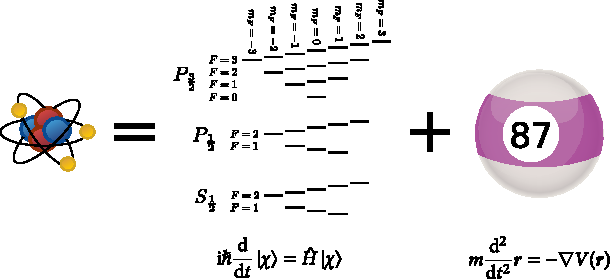
\includegraphics[width=0.75\textwidth]{figures/hidden_variables/semiclassical.pdf}
    \caption{Artist's depiction of a semiclassical atom. Semiclassical models partition the atomic degrees of freedom into those to be modelled quantum mechanically with the Schr\"odinger equation (the electronic degrees of freedom), and those to be modelled with Newtonian mechanics (the motional degrees of freedom). This splits the system into subsystems, which may or may not interact. Some interactions, such as the state-dependent forces of the Stern--Gerlach experiment, are not obvious how to incorporate into such a model given the fundamentally different nature of the two subsystems. Hidden variables can bridge this gap.}
    \label{fig:semiclassical}
\end{figure}

Once one has defined an external potential function $V(\vec r)$ and a Hamiltonian (also possibly varying with space) $\hat H(\vec r)$ for the internal state of the atom, and other possible additions,\footnote{Such as using a Monte-Carlo wavefunction method~\cite{Molmer:93, RevModPhys.70.101} to model the effect of spontaneous emission on $\ket\chi$, and modifying $\vec v$ instantaneously by a random-direction recoil velocity upon each photon emission.} ones job is done and the rest can be left to numerical differential equation solvers to evolve some concrete vector representation $\vec\chi$ of $\ket\chi$ as well as the state variables $\vec r$ and $\vec v$ for motional degree of freedom in time according to the coupled differential equations
\begin{align}\label{eq:simple_semiclassical_first}
\dv{t}\ket\chi &= -\frac\ii\hbar \hat H(\vec r)\ket\chi,\\
\dv{t}\vec v &= -\frac1m\nabla V(\vec r),\\
\dv{t}\vec r &= \vec v\label{eq:simple_semiclassical_last}.
\end{align}
This formulation has been widely successful in simulations of cooling, trapping, and manipulating cold atoms~\cite{mcclelland_atom-optical_1995, wallis_quantum_1995, adams_laser_1997, stenholm_semiclassical_1986, minogin_laser_1987}. In the next subsection I explain why it's not always that simple.

\subsection{Stern--Gerlach separation and evaporative cooling}\label{sec:sterngerlachseparation}

In the Stern--Gerlach experiment~\cite{gerlach_experimentelle_1922}, atoms---with quantum spin and a magnetic moment---were fired as a beam through a region of space with a magnetic field gradient. The well-known result was that two clusters of positions were observed once the beam emerges, rather than a continuous smear of positions, indicating that angular momentum projection---like many quantities in quantum mechanics---is quantised.

This is the case even if one spin-polarises the particles before they are passed through the magnetic field gradient, say putting them in an eigenstate of the $\hat F_x$ operator. Then, if the magnetic field is along the $z$ direction, and the gradient is also in the $z$ direction, two clusters of positions are also observed, even though all particles were in the same state when they entered the region in which there was a magnetic field gradient. This is a display of the indeterminacy of quantum mechanics: even though all particles had the same initial state, there were nonetheless different outcomes for each particle.

The outcome of the Stern--Gerlach experiment is a consequence of quantum mechanics, to be sure, but it has little to do with the wave nature of the atoms themselves. If we introduced some double slits for the atoms to pass through in addition to the magnetic field gradient, then we would be seeing the wave nature of the atoms as interference patterns at the detection screen at the end of the experiment. But if we do not, and if the particles have short de~Broglie wavelengths, then quantum mechanics is not apparent in the motion of the particles through space---except via the influence of spin on seemingly choosing one trajectory or the other. The effect is well understood quantum mechanically, but is difficult to model semiclassically because even if we are happy to approximate wavepackets as small, the wavepackets do not take a single trajectory. Rather they split into two wavepackets, with the part of the superposition corresponding to one spin projection state (along the direction of the local magnetic field) moving one way, and the part of the superposition with the other spin projection going the other way. The trajectories can still be quite classical, it's just that there are two of them.

A similar situation exists in \textsc{rf} evaporative cooling (Section~\ref{sec:evaporative_cooling}) of cold atoms en-route to \textsc{bec}. A common configuration is a magnetic quadrupole trap, with atoms spin-polarised so as to be fully spin-down (for $^{87}$Rb this is the trapped state) with respect to the local magnetic field at the position of each atom. The magnetic field direction---and magnitude---vary in space, and so the spin vectors of different atoms point in different directions in space, but they are all spin-down with respect to the quantisation axis of their local magnetic field. As the atoms move through space, they move in orbits---punctuated by collisions---about the magnetic field zero at the centre of the trap, since they feel a force $F\propto-\nabla\abs{\vec B}$ due to the gradient of the Zeeman potential. Provided they are moving slowly (specifically, provided their Larmor frequency is large compared to the rate of rotation of the magnetic field vector as seen by the atom), the atoms' spins adiabatically follow the local field and remain spin-down, even as the field as seen by each atom fully reverses its direction every half orbital period.

Near the centre of the trap where the atoms are moving faster, the fields are small and therefore have large fractional derivatives and lead to large Larmor periods, adiabaticity no longer holds and the atoms may make spin transitions with respect to their local magnetic field. Once an atom passing close to the field zero has evolved into a superposition of spin-projection states with respect to the local field, it is in a situation identical to the initial condition of the Stern--Gerlach experiment, causing the spin-projection components to spatially separate in the magnetic field gradient. The spin-up component is anti-trapped and repelled from the centre of the trap, and the zero spin-projection component (since the ground state of $^{87}$Rb is spin-$1$) feels no force and moves in a straight line. The spin-down component continues on an orbit about the field zero that is just as tight as before, unaffected by the close approach to the field zero other than being reduced in amplitude. Eventually a collision occurs, either with other atoms or with the walls of the vacuum system and the wavefunction collapses to choose one of these options, leading to atoms probabilistically leaving the trap (called Majorana losses~\cite{Majorana1932, PhysRevLett.74.3352}) or remaining trapped. Again, the trajectories can still be quite classical, it's just that there are three of them, and which trajectory is taken is probabilistic.

How can we model these effects semiclassically? Equations~\eqref{eq:simple_semiclassical_first} to~\eqref{eq:simple_semiclassical_last} are not sufficient, because exists no single classical potential $V(\vec r)$ that can describe the motion of the atoms. Rather, the atoms feel a different force depending on which spin state they are in. Just as the Hamiltonian can be a function of space, so can the potential be a function of the internal state of the atom: $V = V(\vec{r}, \ket\chi)$. Ehrenfest's theorem~\cite{Ehrenfest1927} states that
\begin{align}
m\dv[2]{t}\ev{\hat{\vec r}} = - \ev{\nabla \hat V},
\end{align}
where the expectation values are over all degrees of freedom, not just motional. If we approximate a small wavepacket centred at the position $\vec r$ such that $\ev{\hat{\vec r}} = \vec r$ in order to ignore the wave nature of the atoms, this becomes:
\begin{align}
m\dv[2]{t} \vec r = - \nabla \matrixel{\chi}{\hat V(\vec r)}{\chi},
\end{align}
where the operator $\hat V(\vec r)$ now only acts on the subspace of the internal state of the atom, since we have already taken an expectation value over (a small region of) space. Provided all potentials the atom is subjected to are included in the Hamiltonian for its internal state (including any energy offsets that do not
depend explicitly on the internal state), this is nothing but
\begin{align}
m\dv[2]{t} \vec r = - \nabla \matrixel{\chi}{\hat H(\vec r)}{\chi},
\end{align}
where $\hat H$ is the Hamiltonian describing the evolution of the atom's internal state. We now can construct the \emph{Ehrenfest semiclassical method} describing how the \emph{expectation value} of a well localised atom's position evolves with time:

\begin{align}\label{eq:ehrenfest_semiclassical_first}
\dv{t}\ket\chi &= -\frac\ii\hbar \hat H(\vec r)\ket\chi,\\
\dv{t}\vec v &= -\frac1m \nabla \matrixel{\chi}{\hat H(\vec r)}{\chi},\\
\dv{t}\vec r &= \vec v\label{eq:ehrenfest_semiclassical_last}.
\end{align}

The Ehrenfest semiclassical method is the same as the simple semiclassical method~\eqref{eq:simple_semiclassical_first} to~\eqref{eq:simple_semiclassical_last}, except that it has an answer to the question ``What should we use for $V(\vec r)$ when the atom is in a superposition of states that feel different potentials?'', which is ``use the expectation value''. 

This is all well and good if the expectation value of position is a good approximation to the situation being modelled. But in the Stern--Gerlach experiment or a Majorana spin flip in a magnetic trap, the expectation value of position is a poor match to reality. In the Stern--Gerlach experiment beginning with spin-polarised atoms, a trajectory subject to the mean force or potential (which are both zero for a $50:50$ superposition) would land in a single blob in the middle of the screen, rather than two blobs displaced from the centre. In the case of an atom approaching the field zero in a magnetic trap, use of the mean force would result in the atom broadening its orbit somewhat, rather than splitting into multiple possible trajectories (Figure~\ref{fig:evap_problem}). Semiclassical simulations of evaporative cooling performed by Christopher Watkins (unpublished) displayed an unphysical heating of the atom cloud that I believe is due to the Ehrenfest method's inability to model Stern--Gerlach separation. In a real magnetic trap during evaporative cooling to Bose--Einstein condensation, the mean free path is large enough that the part of the wavepackets that are no longer trapped will usually leave the trap without colliding with any other atoms. This means that the energy the untrapped and anti-trapped components have gained (relative to the trapped component) moving away from the field zero is not usually shared with other atoms upon collision---the extra energy leaves with the atoms. However, if a close approach to the magnetic field zero merely means a broadening of the atoms orbit, then the extra energy does not leave as fast, if at all, and can be shared with other atoms via collisions, turning what would have been an atom loss effect into an overall gradual heating of the cloud.\footnote{This is distinct from the real heating that occurs due to relatively lower energy atoms being more susceptible to Majorana spin flips and thus more likely to be lost, increasing the average energy of atoms remaining---a form of `evaporative heating'.} 

\begin{figure}[t]
    \centerfloat
    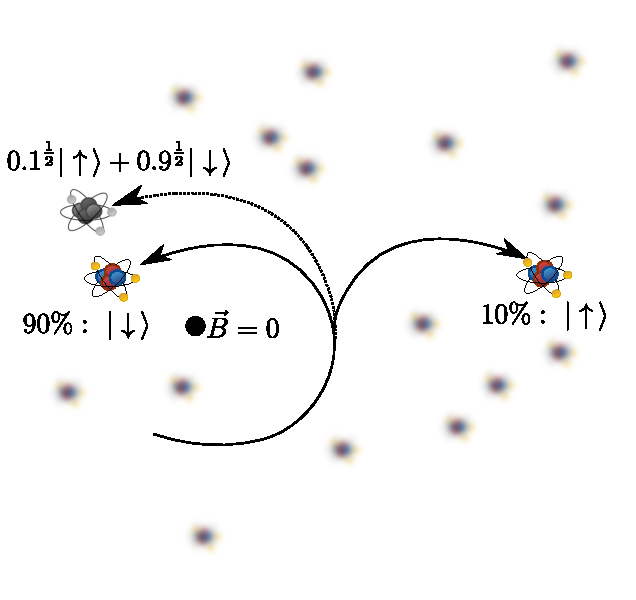
\includegraphics[width=0.75\textwidth]{figures/hidden_variables/evap_problem.pdf}
    \caption{When atoms pass near to the field zero in a magnetic trap, their wavepackets diverge in space as multiple trajectories, each corresponding to one local spin projection state. For example, if a spin-$\frac12$ atom undergoes a partial spin-flip such that it has a ten percent probability of being spin-up, the end result will be two approximate trajectories. One trajectory describes the motion of a wavepacket that is fully spin-up, and one fully spin-down, with the spin-down wavepacket's squared amplitude equal to $0.1$. The Ehrenfest semiclassical method however can only model a single trajectory, and the end result when using this method is a single trajectory being approximately the mean of the two actual trajectories, and retaining a $90:10$ ratio of spin-down:spin-up state populations.}
    \label{fig:evap_problem}
\end{figure}

So how can we modify a semiclassical method to choose only one trajectory? Firstly, since each trajectory corresponds to one of the internal states (though some might be degenerate), our model must choose an internal state and use the classical trajectory corresponding to that internal state only. Secondly, since all atoms begin in identical states and yet some take one trajectory and some another, this choice must be probabilistic. Finally, the probabilities must be consistent with those from quantum mechanics, i.e.~the Born rule~\cite{born_zur_1926}: the probability of an atom taking each trajectory must be proportional to the squared amplitude of the internal state of the atom, projected onto the eigenstate corresponding to that trajectory.

There exists a category of theories dealing with precisely this question of how to choose a specific state of a quantum system in a stochastic way, such that the probability of having chosen a state is equal to that given by quantum mechanics. Such theories are called \emph{hidden-variable} theories, and any parameter, variable or label specifying which state has been chosen is a \emph{hidden variable}.

\section{Hidden-variable theories}\label{sec:hidden_variable_theories}

In his paper \emph{Quantum computing and dynamical quantum models}, Aaronson defines a \emph{dynamical quantum model}~\cite{aaronson_quantum_2002}:

\begin{quote}
A \emph{dynamical quantum model} assigns an eigenstate to a specified observable even when no measurement is made, and gives a stochastic evolution rule for that eigenstate. Such a model yields a distribution of classical histories of a quantum state.
\end{quote}
In a later paper, \emph{Quantum computing and hidden variables}, superseding the first, Aaronson renames dynamical quantum models to \emph{hidden-variable theories} and refines the definition~\cite{PhysRevA.71.032325}:
\begin{quote}
For us, a hidden-variable theory is simply a way to convert a unitary matrix that maps one quantum state to another, into a stochastic matrix that maps the initial probability distribution to the final one in some fixed basis.
\end{quote}
I adopt this definition of a hidden-variable theory for the purposes of this thesis.

The language of the first definition is more tangible for us---we wish to \emph{assign an eigenstate} to our atoms (choose one of the internal states in order to decide which trajectory to follow), and have a \emph{stochastic evolution rule} for which eigenstate is chosen at any one time (allow the atom to begin taking a different trajectory if it makes transitions between states), probabilistically depending on the change in quantum populations of the states. But the second definition is more specific: the stochastic evolution rule is in the form of a stochastic matrix, with elements equal to transition probabilities for some time interval. And the rule should be in some way based on the unitary evolution that the quantum system evolves according to in the same interval of time, such that the initial and final probabilities of the stochastic matrix and unitary evolution agree. That is, if a quantum state $\ket\chi$ evolves in a certain basis $\{\ket{\chi_i}\}$according to a unitary $\hat U(t^\prime, t)$:
\begin{align}
\left[\begin{matrix}
c_1(t^\prime)\\c_2(t^\prime)\\c_3(t^\prime)\\\vdots
\end{matrix}\right]
= \left[\begin{matrix}
U_{11}(t^\prime, t) & U_{12}(t^\prime, t) & U_{13}(t^\prime, t)&\hdots\\
U_{21}(t^\prime, t) & U_{22}(t^\prime, t) & U_{23}(t^\prime, t)&\hdots\\
U_{31}(t^\prime, t) & U_{32}(t^\prime, t) & U_{33}(t^\prime, t)&\hdots\\
\vdots & \vdots & \vdots & \ddots
\end{matrix}\right]
\left[\begin{matrix}
c_1(t)\\c_2(t)\\c_3(t)\\\vdots
\end{matrix}\right],
\end{align}
where $c_i = \braket{\chi_i}{\chi}$ and $U_{ij}(t^\prime, t) = \matrixel{\chi_i}{\hat U(t^\prime, t)}{\chi_j}$, then a hidden-variable theory is a matrix-valued function $S(U(t^\prime, t), \vec\chi(t)))$, where $\vec\chi(t)$ and $U(t^\prime, t)$ are the vector and matrix representations of the state vector $\ket{\chi(t)}$ and unitary $\hat U(t^\prime, t)$ in the $\{\ket{\chi_i}\}$ basis, that satisfies\footnote{In order to more clearly compare to quantum evolution, we are using \emph{left stochastic} matrices, which multiply column vectors of probabilities from the left, contrary to the most common convention for stochastic matrices, which is to multiply row matrices from the right. Thus $S$ has unit column sums, whereas the corresponding right stochastic matrix (its transpose) would have unit row sums.}
\begin{align}
\left[\begin{matrix}
\abs{c_1(t^\prime)}^2\\\abs{c_2(t^\prime)}^2\\\abs{c_3(t^\prime)}^2\\\vdots
\end{matrix}\right]
= \left[\begin{matrix}
S_{11}(t^\prime, t) & S_{12}(t^\prime, t) & S_{13}(t^\prime, t)&\hdots\\
S_{21}(t^\prime, t) & S_{22}(t^\prime, t) & S_{23}(t^\prime, t)&\hdots\\
S_{31}(t^\prime, t) & S_{32}(t^\prime, t) & S_{33}(t^\prime, t)&\hdots\\
\vdots & \vdots & \vdots & \ddots
\end{matrix}\right]
\left[\begin{matrix}
\abs{c_1(t)}^2\\\abs{c_2(t)}^2\\\abs{c_2(t)}^2\\\vdots
\end{matrix}\right].
\end{align}
In essence, if quantum unitary evolution maps complex state amplitudes to complex state amplitudes, a hidden-variable theory maps probabilities to probabilities. Thus the elements of $S$ can be used as conditional probabilities---or transition probabilities---for a hidden variable $\eta(t)$: a piecewise-constant function of time with values equal to a state index, label, or quantum number that uniquely identifies one eigenstate at each moment in time. $\eta(t)$ evolves stochastically, with the elements of $S$ giving the chance that the state $\ket{\chi_\eta} \in \{\ket{\chi_i}\}$ assigned by the hidden variable will change from one to another in a given time interval:
\begin{align}\label{eq:conditional_probability}
\Pr(\eta(t^\prime){=}i|\eta(t){=}j) = S_{ij}(U(t^\prime, t), \vec\chi(t)).
\end{align}

We are interested in such hidden variable theories because they can wrap a layer of classical interpretation around quantum evolution. In a semiclassical model, the internal state of an atom is modelled quantum mechanically, such that $\vec\chi(t)$ and $U(t^\prime, t)$ are known at every timestep. A stochastic hidden-variable theory can take these quantities---a description of the quantum evolution at each timestep---and give us back transition probabilities that allow us to evolve a hidden variable $\eta(t)$. This hidden variable's value at any moment in time will be equal to the label, index or quantum number of one state in the chosen basis, with probability equal to that state's population. Since each eigenstate of the Hamiltonian is subject to a well-defined adiabatic potential, the hidden variable can be used to connect the quantum evolution of the atom's internal state to the requirement that the classical motion use a single, well-defined force at each moment. And it can do so in a way consistent with the quantum probabilities of the internal state.

There are many ways to define functions $S$ that satisfy the condition~\eqref{eq:conditional_probability}. The simplest is to ignore the unitary completely and set $S_{ij} = \abs{c_i(t^\prime)}^2$, which yields:
\begin{align}
\Pr(\eta(t^\prime){=}i|\eta(t){=}j) = \abs{c_{i}(t^\prime)}^2,
\end{align}
that is that the hidden variable $\eta$ is equally likely to transition to a given value regardless of its previous value, and regardless of the unitary, and that the conditional transition probability from all input states is just the squared amplitude of the final state. This theory represents a hidden variable that jumps between states randomly based on their population, with no regard for its history or whether there were actually amplitude flows between the states between which it is transitioning. Nonetheless, this theory, called \emph{product theory}~\cite{PhysRevA.71.032325}, matches the definition of a hidden-variable theory---$S$ is a stochastic matrix, and the hidden variable on average will spend an amount of time in each state consistent with the Born rule.

In order to further classify hidden-variable theories with respect to whether they have this or other kinds of strange behaviour, Aaronson outlines some additional axioms~\cite{PhysRevA.71.032325} that hidden variables ought to satisfy---in addition to reproducing the Born rule---including reasonable statements about symmetries, and insensitivity to small perturbations. He goes on to prove that the axioms cannot all be satisfied simultaneously---all hidden-variable theories have some undesirable property or another---but he shows some theories satisfy more axioms than others.

It is convenient to introduce the matrix $P$ of absolute (unconditional) transition probabilities.\footnote{By unconditional probabilities, I mean the probabilities of the hidden variable transitioning between pairs of states, given no knowledge of which state was selected prior to transitioning.} Summing~\eqref{eq:conditional_probability} over all possible initial values of the hidden variable yields the probability of it having a particular final value after the given time interval:
\begin{align}
\Pr(\eta(t^\prime){=}i) 
= \sum_j \Pr(\eta(t^\prime){=}i|\eta(t){=}j) \Pr(\eta(t){=}j),
\end{align}
which, recognising that the final and initial probabilities must be the final and initial squared amplitudes of the state vector, can be rewritten:
\begin{align}
\abs{c_i(t^\prime)}^2
= \sum_j S_{ij}(U(t^\prime, t), \vec\chi(t)) \abs{c_j(t)}^2.
\end{align}
We now define the matrix of absolute transition probabilities $P$:
\begin{align}\label{eq:P_matrix_def}
P_{ij} = S_{ij}(U(t^\prime, t), \vec\chi(t)) \abs{c_j(t)}^2,
\end{align}
such that:
\begin{align}
\abs{c_i(t^\prime)}^2
= \sum_j P_{ij}.
\end{align}
So we have that $P$ has row sums equal to the final squared amplitudes.
And, because $P_{ij} = S_{ij}\abs{c_j(t)}^2$ and $S$ is a stochastic matrix with column sums equal to one, we have that $P$ must have row sums equal to the initial squared amplitudes.

Now that we have introduced $P$ and shown what its row and column sums must be, we come to a particularly simply defined hidden-variable theory called Schr\"odinger theory,\footnote{Not to be confused with the wave mechanics governed by the Schr\"odinger wave equation, the arbiter of success for the models presented in this chapter.} discussed in Aaronson's hidden variables paper~\cite{PhysRevA.71.032325}. The idea is to form $P$ by starting with the matrix of absolute values of $U$, and simply scaling its rows and columns to have the correct values:\footnote{One might expect that the absolute value squared might be a better choice, since this matches Fermi's golden rule. Aaronson discusses in his paper, when presenting his own hidden-variable theory \emph{Flow theory}, how absolute values of elements of the unitary have some appealing properties.}
\begin{align}
P = \left[\begin{matrix}
a_1b_1\abs{U_{11}(t^\prime, t)} & a_1b_2\abs{U_{12}(t^\prime, t)} & a_1b_3\abs{U_{13}(t^\prime, t)}&\hdots\\
a_2b_1\abs{U_{21}(t^\prime, t)} & a_2b_2\abs{U_{22}(t^\prime, t)} & a_2b_3\abs{U_{23}(t^\prime, t)}&\hdots\\
a_3b_1\abs{U_{31}(t^\prime, t)} & a_3b_2\abs{U_{32}(t^\prime, t)} & a_3b_3\abs{U_{33}(t^\prime, t)}&\hdots\\
\vdots & \vdots & \vdots & \ddots
\end{matrix}\right],
\end{align}
that is,
\begin{align}
P_{ij} = a_i b_j \abs{U_{ij}(t^\prime, t)},
\end{align}
where the row scalings $\{a_i\}$ and column scalings $\{b_j\}$ satisfy:
\begin{align}
\sum_j a_i b_j \abs{U_{ij}(t^\prime, t)} = \abs{c_i(t^\prime)}^2,\label{eq:a_scalings}\\
\sum_i a_i b_j \abs{U_{ij}(t^\prime, t)} = \abs{c_j(t)}^2\label{eq:b_scalings},
\end{align}
which can be solved numerically, and then the Schr\"odinger theory stochastic matrix then able to be extracted by inverting~\eqref{eq:P_matrix_def}:
\begin{align}\label{eq:schrodinger_S_matrix}
S_{ij}(U(t^\prime, t), \vec\chi(t))
= a_i b_j \frac{\abs{U_{ij}(t^\prime, t)}}{\abs{c_j(t)}^2}.
\end{align}

Schr\"odinger theory is the hidden-variable theory I have used in the simulations in the results section of this chapter (Section~\ref{sec:HVSC_results}). In Section~\ref{sec:schrodinger_theory_numerics} I detail my efforts to most efficiently find the row and column scalings in order to actually compute the Schr\"odinger theory $S$ matrix.

The choice to use Schr\"odinger theory for the simulations was made prior to my learning of Tully's fewest-switches algorithm in the surface-hopping literature~\cite{doi:10.1063/1.459170, doi:10.1146/annurev-physchem-040215-112245, doi:10.1063/1.2715585} (also detailed in Section~\ref{sec:fewest_switches}), and fewest-switches has a number of properties that make it more appealing than Schr\"odinger theory for use in a hidden-variable semiclassical/surface-hopping simulation. Tully's fewest-switches has three main advantages. The first is its low computational cost, whereas (as detailed in Section~\ref{sec:schrodinger_theory_numerics}) Schr\"odinger theory is considerably more computationally expensive to evaluate (except in the case of a two-state system). The second, which is only relevant for time-dependent Hamiltonians, is that fewest-switches can be formulated in a way that allows a distinction to be drawn between motion of a particle through an inhomogeneous field as the cause of non-adiabatic transitions, versus non-adiabatic transitions being caused by explicitly time-dependent fields. I conjecture on the usefulness of this distinction in Sections~\ref{sec:fewest_switches} and~\ref{sec:velocity_correction}. The final advantage is in the name: fewest-switches makes the \emph{fewest number of switches} consistent with the quantum probabilities in each infinitesimal time interval, whereas Schr\"odinger theory makes more switches. That is, the transition probabilities in fewest-switches are smaller than those in Schr\"odinger theory, causing the hidden variable to make fewer transitions in the former than the latter. More switches means larger statistical variation in the outcomes: even though the expectation value of the number of atoms in each state are consistent with the Born rule, the variance is higher, and a larger ensemble will be required to see agreement with the Born rule within some tolerance. More switches also implies larger statistical variation in the classical trajectories, as it increases the chance that atoms have followed multiple classical trajectories in a region of non-adiabatic coupling than followed just one. As mentioned in the introduction to this chapter, Schr\"odinger theory has one advantage over fewest-switches: it allows one to compute transition probabilities corresponding to quantum evolution over an arbitrary time interval, so long as one has the unitary that describes that evolution. Fewest-switches, on the other hand, produces differential probabilities that must be integrated over time to obtain transition probabilities over intervals that are long compared to the dynamical timescales of the problem. This is usually not a problem since one typically evolves the state vector using timesteps shorter than dynamical timescales of the problem. However Schr\"odinger theory could still be useful for problems where the quantum evolution can be performed analytically, and where computing transition probabilities at repeated intervals is the limiting factor in the size of simulation timesteps.

\section{Overview of method}\label{sec:overview_of_method}

\begin{figure}[t]
    \centerfloat
    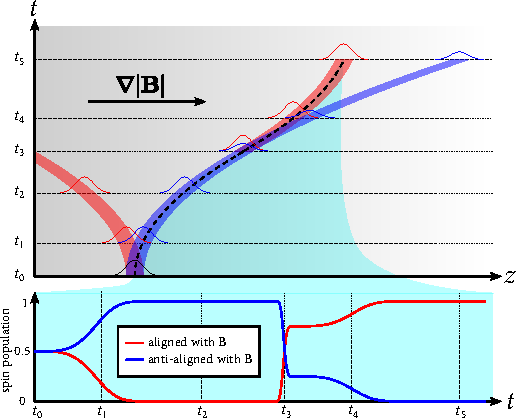
\includegraphics{figures/hidden_variables/schematic.pdf}
    \caption{Schematic of the method. At $t_0$ an atom is in a $50$:$50$ superposition of spin-up:spin-down population, and the two spin components accelerate apart in the magnetic field gradient. If the hidden variable dictates that we follow the spin-down component (the initial trajectory given by the dotted line), then we see a reduced spin-up population at times $t_1$ and $t_2$. At $t_3$ the field changes direction suddenly, and partly flips the spins (in the local basis with quantisation axis given by the direction of the magnetic field). The stochastic hidden variable transitions to instead select the spin-up component, which we follow thereafter. Following the spin-up component we then see the a reduced spin-down population at $t_5$ due to the wavepackets separating once more.}\label{fig:HVSC_schematic}
\end{figure}

To motivate the method and highlight some necessary properties of a sensible semiclassical model capable of simulating Stern--Gerlach separation, consider, as an example, a spin-$\frac12$ particle undergoing separation in a magnetic field gradient. The two spin components accelerate away from each other, with the relative acceleration vector pointing in the same direction as the gradient in field strength. We can ask the question: ``What spin-state populations would I see, if I followed the spin-down wavepacket only?" The meaning of `follow' will be made more precise in Section~\ref{sec:decoherence}, but for now we will simply look at the spin populations in the vicinity of the region of space occupied by the spin-down wavepacket.

As shown in~\figref{fig:HVSC_schematic}, one sees the spin-up population decreasing over time until only spin-down population remains. The rate at which spin-up population `leaves' the region of space we are watching depends on how quickly the wavepackets are accelerating away from each other, as well as the shape of the wavepackets. Likewise, if one follows the spin-up component instead, one sees the spin-down population decrease to zero.

Motivated by this observation, the hidden-variable semiclassical method is a phenomenological model comprised of the following:
\begin{itemize}
\item{One internal state of the atom is chosen at any moment in time, stored along with the state vector as a stochastic hidden variable that can make a transition at each timestep, according to a hidden-variable theory. The hidden-variable theory takes as input the state vector, and the Hamiltonian or unitary evolution matrix describing the evolution of the internal state of the atom at each timestep. By evolving according to a hidden-variable theory, the probability of the hidden variable selecting a particular internal state is equal to that state's population at each moment in time.}
\item{The internal state of the atom evolves according to the Schr\"odinger equation, but with the addition of back-action caused by the continuous projection of the atomic wavefunction onto a specific `classical' motional state under assumptions about the form and evolution of all motional states. This is a vexed matter to which I devote several sections later in this chapter.}
\item{Upon a change in the state selected by the hidden variable, the velocity of the atom is modified instantaneously as required by energy conservation, or, if this would result in a negative kinetic energy, the transition is disallowed.}
\end{itemize}

Written in the same way as in Section~\ref{sec:semiclassical_methods}, the model amounts to the following coupled differential equations and stochastic transition rule:
\begin{align}\label{eq:eq:hvsc_semiclassical_simple_first}
\dv{t}\ket{\tilde\chi} &= -\frac\ii\hbar \hat H(\vec r, t)\ket{\tilde\chi} - \hat\Gamma_\eta(\vec r, t)\ket{\tilde\chi},\\
\dv{t}\vec v &= -\frac1m\nabla V_\eta(\vec r, t),\\
\dv{t}\vec r &= \vec v\\
\Pr(\eta(t^\prime){=}i|\eta(t){=}j) &= S_{ij}(U_\up{eff}(t^\prime, t), \vec\chi(t)),
\label{eq:hvsc_semiclassical_simple_last}
\end{align}
where $\ket{\tilde\chi}$ is the internal state vector including the effect of back-action (neglecting normalisation), $\hat\Gamma_\eta(\vec r, t)$ is a non-Hermitian operator that implements this back-action by decaying the amplitude of states not being followed (there are many ways to do this, all approximate, discussed in Section~\ref{sec:decoherence}), $\eta$ is the hidden variable, $V_\eta$ is the adiabatic potential experienced by the eigenstate selected by the hidden variable, $\vec\chi$ is the vector representation of the (normalised) state vector in the local eigenbasis, and $U_\up{eff}(t^\prime, t)$ is the unitary matrix describing the evolution of the state vector from time $t$ to $t^\prime$ in the local eigenbasis under the action of the effective Hamiltonian $\hat H_\up{eff}$, defined in Section~\ref{sec:fewest_switches}. In addition to these evolution rules, the state vector must be normalised at each timestep of simulation,\footnote{It would be relatively simple to include a term in the differential equation to preserve normalisation, but the non-normalisation-preserving differential equation is simpler to write, compute, and understand.} and the velocity of the atom modified instantaneously whenever a transition is made in order to conserve energy. This latter requirement is detailed in Section~\ref{sec:velocity_correction}.

\section{Hidden variables: implementation details}\label{sec:implementation_details}

In this section I go into the gritty details of numerically evaluating hidden-variable theories, conserving energy when a transition occurs, and some other concerns.

\subsection{Numerically evaluating Schr\"odinger theory}\label{sec:schrodinger_theory_numerics}

Despite the high computational cost of Schr\"odinger theory relative to Tully's fewest-switches, here I present the results of my investigation into how to minimise said cost. There are many ways to numerically solve for the row and column scalings $\{a_i\}$ and $\{b_i\}$ required to compute the $S$ matrix of Schr\"odinger theory~\eqref{eq:schrodinger_S_matrix}, but there is one unique solution for the resulting scaled matrix $S$.\footnote{The values of $\{a_i\}$ and $\{b_j\}$ are only determined up to an overall multiplication of each $\{a_i\}$ by a constant and division of each $\{b_j\}$ by the same constant, since only products $a_i b_j$ appear in the resulting scaled matrix.} The simplest method is to simply alternate between scaling the rows to get the right row sums, then scaling the columns to get the right column sums, and repeating, that is, alternating between solving~\eqref{eq:a_scalings} for all $a_i$, and solving~\eqref{eq:b_scalings} for all $b_i$, until the result converges. This is called the Sinkhorn--Knopp method of r-c (row-column) scaling~\cite{knight_sinkhornknopp_2008}, but is computationally intensive, with slow convergence~\cite{Linial2000}. An alternative is the method by Linial \emph{et al.}~\cite{Linial2000} which converges much faster. Both are iterative methods, and so in practice one can save the resulting row and column scalings at each integration step of a simulation and use them as the initial guesses for the same computation at the next integration step,\footnote{With the caveat that since the row and column scalings are only determined up to an overall multiplication/division, occasional multiplication of all $\{a_i\}$ and division of all $\{b_i\}$ by a constant may be necessary to prevent the values numerically overflowing or underflowing in the middle of a simulation.} providing a considerable speedup.

For the case of a two-state system, the row and column scalings can be found analytically, with the result
\begin{align}
a_1 &= 1\\
a_2 &: a_2^2 + 
\left(\frac1{AB} - \frac AB \abs{c_1(t)}^2 - \frac BA \abs{c_2(t)}^2\right)a_2
+ \frac{\abs{c_2(t^\prime)}^2}{\abs{c_1(t^\prime)}^2} = 0;\ a_2 > 0\\
b_1 &= \frac{\abs{c_1(t^\prime)}^2}{A + B a_2}\\
b_2 &= \frac{\abs{c_2(t^\prime)}^2}{B + A a_2},
\end{align}
where $A = \abs{U_{11}} = \abs{U_{22}}$ and $B = \abs{U_{12}} = \abs{U_{21}}$. This result only holds in the case of Schr\"odinger theory for a state vector with two components subject to unitary evolution---not for row-column scaling in general---since it makes use of symmetries of unitary matrices and the fact that the initial and final probabilities given by the squared amplitudes of the state vector components must sum to unity.

Some further notes on numerics: the above expressions for Schr\"odinger theory and its analytic expression for a two-state system involve dividing by elements of the unitary, and by state populations, both of which may be zero or very close to zero. Whilst the relevant limits may exist, we cannot easily compute them numerically, and so I have taken to simply replacing small values of $\abs{U_{ij}}$, $\abs{c_i(t^\prime)}^2$ and $\abs{c_j(t)}^2$ with a tiny non-zero constant (I use $\varepsilon=10^{-100}$), ensuring that the convergence criterion (which represents a tolerance for the sum squared error in the column sums) I pass to Linial's method is larger than the square of this by some margin, so as to allow convergence even though modifying the matrix elements may make the matrix no longer row-column scalable to higher precisions. I use a convergence criterion of $10^{-16}$ for Linial's algorithm, implying the root sum squared error in column sums will be at most $10^{-8}$, which is small compared to unity---the sum of all column sums for a perfectly scaled matrix given that the column sums are probabilities that must add to unity. Smaller tolerances imply more iterations before convergence, so tolerances should be as large as is acceptable for the problem if computational cost is a limiting factor.

Potentially faster algorithms exist for row-column scaling of matrices,\footnote{In my simulations for realistic $3\times3$ unitaries corresponding to evolution over small time intervals, Linial's method converges to the aforementioned tolerance in about $100-200$ iterations, taking about $20-40\unit{\upmu s}$ per matrix on a $2.9\unit{GHz}$ 7$^\up{th}$ generation Intel core i7 \textsc{CPU}. This is when transitions are actually occurring; before and after periods of non-adiabatic evolution the algorithm converges in zero or one step when the unitary is the identity and the state vector is in a single eigenstate.} for example, approaches that treat the problem one of root-finding or optimisation aimed at solving the simultaneous equations~\eqref{eq:a_scalings} and~\eqref{eq:b_scalings} or minimising their sum squared error~\cite{knight_fast_2013}. When prototyping with small ($3\times 3$) random unitary matrices and random state vectors, I found Newton's method to be effective at quickly solving this set of equations (after fixing $a_1=1$ to make them fully determined), requiring considerably fewer iterations that Linial's method. However, the unitaries and state vectors in quantum mechanics are not random, and the fact that most elements of the unitary and state vector are zero when there is no evolution and the atom is in an eigenstate resulted in numerical difficulties with Newton's method that Linial's method does not seem to encounter. Similar to many of the methods in reference~\cite{knight_fast_2013}, one could construct a hybrid method that takes a Newton step, and then checks the row sum and column sum residuals, and if they increased compared to the previous step, ignores that step and takes a step of Linial's method instead. I have not attempted this, and for the moment use Linial's method.

A final note is that my hidden-variable semiclassical method is not only agnostic to which matrix scaling algorithm is used, but that it is also not married to any particular hidden-variable theory. An early version of the method~\cite{billington_monte_2015} was limited to two-component systems, and the probability of transition was computed as
\begin{align} 
\Pr(\eta(t^\prime){=}2|\eta(t){=}1) &=
\max\left(0, \abs{c_2(t^\prime)}^2 - \abs{c_2(t)}^2\right),\\
\Pr(\eta(t^\prime){=}1|\eta(t){=}2) &= 
\max\left(0, \abs{c_1(t^\prime)}^2 - \abs{c_1(t)}^2\right),
\end{align}
that is, I simply inspected the populations each step and declared any positive change in population of a state as a probability of transition from the other state. Since there were only two states, the originating state of the transition was unambiguous, but the method did not generalise to systems with three or more states.\footnote{This was before I coincidentally came across the definition of a stochastic hidden-variable theory in Aaronson's book \emph{Quantum computing since Democritus}~\cite{aaronson_quantum_2013} and realised that what I had made was a hidden-variable theory, allowing me to choose a more general one from his paper (and before later still, finding Tully's fewest-switches algorithm).} However, it resulted in simulated final populations that on average agreed with the underlying Schr\"odinger wave equation, leading me to suspect that the exact hidden-variable theory used is not crucial, so long as it satisfies the most obvious of Aaronson's axioms so as not to behave like the product theory mentioned in Section~\ref{sec:hidden_variable_theories}. I chose Schr\"odinger theory fairly arbitrarily, it being the one that seemed most easily computable out of the two presented in Aaronson's paper~\cite{PhysRevA.71.032325}, but one might try using Aaronson's flow theory, or inventing another altogether. The surface-hopping literature uses Tully's fewest-switches algorithm with much success, as well as approximations to it~\cite{FABIANO2008111} that are even cheaper, computationally speaking.

Interestingly, the main conclusion of Aaronson's paper~\cite{PhysRevA.71.032325} is that if we could know the entire history of a hidden variable, we could use it to make a computer more powerful than a quantum computer. It is therefore perhaps not surprising that hidden-variable theories ought to be computationally expensive to simulate on a classical computer. Prior to discovering Tully's fewest-switches algorithm, I was therefore somewhat resigned to the fact that any hidden-variable theory would likely be computationally expensive to compute. In light of this it was pleasantly surprising to discover that Tully's fewest-switches (discussed in the next subsection) is computationally cheap. The seeming conflict could be reconciled however if the computational power of hidden variables is crucially dependent on some feature we are not interested in and which fewest-switches does not capture, such as agreement with arbitrary unitaries rather than only those due to evolution over small time intervals, as is assumed by fewest-switches.

\subsection{Time-dependent formulation of Tully's fewest-switches algorithm}\label{sec:fewest_switches}

In this subsection I derive Tully's fewest-switches algorithm~\cite{doi:10.1146/annurev-physchem-040215-112245, doi:10.1063/1.459170} with the extension that the Hamiltonian may have arbitrary time-dependence. As such, the non-adiabatic transitions that can occur can be due to either the spatial variation of the Hamiltonian, or its time variation. It is important identify which of the two non-adiabatic effects is responsible for a given transition of the hidden variable, as energy conservation only applies to transitions due to spatial variation, whereby the atom is paying/receiving the energy cost of a transition using its kinetic energy. However for a transition due to temporal variation of the Hamiltonian, energy can be added and removed from the atom by the driving field without conserving its total energy. I propose that velocity corrections therefore ought to only be performed following transition of the hidden variable if that transition was due to spatial variation in the Hamiltonian, and not temporal variation.\footnote{One cannot simply compute the (partial) time derivative of the Hamiltonian's eigenvalues and multiply by $\upDelta t$ to infer the energy change over one timestep, as the actual transition takes place over many timesteps, despite the hidden variable transitioning during a single timestep. This disconnect is the fundamental source of difficulty in correctly conserving energy in these models.}

This proposed extension to fewest-switches is speculative and untested---in Section~\ref{sec:HVSC_results} I present results of the model for the case of time-independent fields only. It is clear that the extension would yield the correct behaviour in both the limit of a time-independent inhomogeneous field (energy is always conserved via velocity jumps) and a time-dependent homogeneous field (energy is never required to be conserved and there are no velocity jumps), though its suitability in the intermediate regime is less clear without comparing simulation results to the Schr\"odinger wave equation.

This subsection also serves to present Tully's fewest-switches algorithm and the concepts and notation related to it that I refer to in later sections.

We begin with the time-dependent Schr\"odinger equation for the internal state $\ket{\chi(t)}$ of an atom at position $\vec r$:
\begin{align}
\ii\hbar\dv{t}\ket{\chi(t)} = \hat H(\vec r, t)\ket{\chi(t)}\label{eq:Tully_schro}
\end{align}
Now we take the unitary $\hat U_H(\vec r, t)$ that transforms state vectors into the eigenbasis of $\hat H$ such that
\begin{align}\label{eq:U_H_definition}
\hat H(\vec r, t) = \hat U_H^\dagger(\vec r, t) \hat V(\vec r, t) \hat U_H(\vec r, t),
\end{align}
where $\hat V(\vec r, t)$ is a diagonal operator with diagonals equal to the adiabatic potentials that each eigenstate of $\hat H$ is subject to in the adiabatic approximation.
We can therefore define the state vector in the adiabatic picture for $\hat H$ as\footnote{This is very similar to an interaction picture state vector (Section~\ref{sec:interaction_picture}), but as I have previously used the definition of an interaction picture as the transformation that diagonalises a \emph{time-independent} Hamiltonian, this potentially time-dependent Hamiltonian does not satisfy the definition.}
\begin{align}\label{eq:chi_Hbasis}
\ket{\chi_H(t)} &= \hat U_H(\vec r, t)\ket{\chi(t)}\\
\Rightarrow \ket{\chi(t)} &= \hat U^\dagger_H(\vec r, t)\ket{\chi_H(t)}.
\end{align}
Substituting~\eqref{eq:chi_Hbasis} into~\eqref{eq:Tully_schro} and premultiplying by $\hat U_H(\vec r, t)$ yields
\begin{align}
\ii\hbar\hat U_H(\vec r, t)\dv{t}\hat U^\dagger_H(\vec r, t)\ket{\chi_H(t)} = \hat U_H(\vec r, t)\hat H(\vec r, t)\hat U^\dagger_H(\vec r, t)\ket{\chi_H(t)},
\end{align}
which via the product rule and our definition of $\hat V(\vec r, t)$ simplifies to the differential equation obeyed by the transformed state vector $\ket{\chi_H(t)}$:
\begin{align}\label{eq:Tully_adiabatic_schro}
\ii\hbar\dv{t}\ket{\chi_H(t)} &= \left[
  \hat V(\vec r, t)
  - \ii\hbar\hat U_H(\vec r, t)\dv{t}U^\dagger_H(\vec r, t)
 \right]\ket{\chi_H(t)}\\
 &\equiv \hat H_\up{eff} \ket{\chi_H(t)}.\label{eq:Tully_adiabatic_eff}
\end{align}
This equation has the same form as the Schr\"odinger equation, with the contents of the brackets comprising an effective Hamiltonian dictating the dynamics of the state vector in the \emph{adiabatic basis} (the basis in which $\hat H$ is diagonal). Like a non-inertial reference frame in classical mechanics, use of this transformed basis has resulted in the appearance of an extra term in the Hamiltonian, the non-adiabatic coupling term depending on the time derivative of the transformation $\hat U_H^\dagger$.

Here we differ from Tully by proceeding without assuming that $\hat U_H$ has no explicit time dependence. The total time derivative of $\hat U_H^\dagger$ includes both its direct time dependence and the effect of motion through space; the latter obtainable via the chain rule:
\begin{align}
\dv{t}\hat U^\dagger_H(\vec r, t)
 = \pdv{t} \hat U^\dagger_H(\vec r, t) + \vec v\cdot \nabla \hat U^\dagger_H(\vec r, t),
\end{align}
where $\vec v = \dv{\vec r}{t}$. Thus~\eqref{eq:Tully_adiabatic_schro} becomes:
\begin{align}\label{eq:Tully_adiabatic_schro_simplified}
\ii\hbar\dv{t}\ket{\chi_H(t)} = \left[
  \hat V(\vec r, t)
  - \ii\hbar\hat U_H(\vec r, t)\pdv{t} \hat U^\dagger_H(\vec r, t)
   - \ii\hbar\vec v\cdot \hat U_H(\vec r, t)\nabla \hat U^\dagger_H(\vec r, t)
 \right]\ket{\chi_H(t)}.
\end{align}
The final term is identical to the non-adiabatic coupling term in the equation of motion as usually written in the surface-hopping literature~\cite{doi:10.1146/annurev-physchem-040215-112245} being a matrix with elements (in the eigenbasis):
\begin{align}
\left(- \ii\hbar\vec v\cdot U_H(\vec r, t)\nabla U^\dagger_H(\vec r, t)\right)_{ij}
= - \ii\hbar\vec v\cdot\matrixel{\chi_i(\vec r, t)}{\nabla}{\chi_j (\vec r, t)},
\end{align}
where $U_H(\vec r, t)$ is the matrix representation of $\hat U_H$ in any basis that does not vary spatially (i.e.~not the eigenbasis), $\ket{\chi_i(\vec r, t)}$ is the $i^\up{th}$ eigenvector of $\hat H(r, t)$, and $\matrixel{\chi_i(\vec r, t)}{\nabla}{\chi_j (\vec r, t)}$ is the \emph{non-adiabatic coupling vector} between the $i^\up{th}$ and $j^\up{th}$ states referred to in the literature~\cite{doi:10.1146/annurev-physchem-040215-112245}. The second to last term in brackets in~\eqref{eq:Tully_adiabatic_schro_simplified}
is the additional contribution due to the time-dependence of the Hamiltonian (more specifically, the time-dependence of its eigenbasis).

We now proceed identically to Tully, computing the rate of change of an eigenstate's population $\abs{c_i(t)}^2$ as
\begin{align}
\dv{t}\abs{c_i(t)}^2 = c_i(t) \dv{t}c_i^*(t) + c_i^*(t) \dv{t}c_i(t),
\end{align}
where via~\eqref{eq:Tully_adiabatic_schro_simplified} we have:
\begin{align}
\dv{t}c_i(t) &= -\frac\ii\hbar\sum_j \left(H_\up{eff}(\vec r, t)\right)_{ij} c_j(t)\\
\Rightarrow \dv{t}c_i(t) &= -\frac\ii\hbar \sum_j\left[V_{ij}(\vec r, t)
  - \ii\hbar\matrixel{\chi_i(\vec r, t)}{(\partial_t + \vec v\cdot\nabla)}{\chi_j(\vec r, t)}
 \right] c_j(t).
\end{align}
This yields the time rate of change of the population $\abs{c_i(t)}^2$:
\begin{align}
\dv{t}\abs{c_i(t)}^2 &= \left[-\frac\ii\hbar \sum_j c_i^*(t) \left(H_\up{eff}(\vec r, t)\right)_{ij} c_j(t)\right] + \up{c.c.}\\
&= -\frac2\hbar\sum_j\im\left(c_i^*(t) \left(H_\up{eff}(\vec r, t)\right)_{ij} c_j(t)\right)\label{eq:fewest_switches_Heff}\\
&= -\frac2\hbar\sum_j\im\left(c_i^*(t)
\left[V_{ij}(\vec r, t)
  - \ii\hbar\matrixel{\chi_i(\vec r, t)}{(\partial_t + \vec v\cdot\nabla)}{\chi_j(\vec r, t)}
 \right]
 c_j(t)\right).
\end{align}
Since $V(\vec r, t)$ is diagonal\footnote{This is not always assumed in the surface-hopping literature, since additional couplings are sometimes included in $V$ which have not been removed by diagonalisation.} and real, $c_i^*(t)V_{ij}(\vec r, t)c_j(t)$ is zero when $i\neq j$, and has no imaginary part when $i=j$, leaving us with
\begin{align}
\dv{t}\abs{c_i(t)}^2 &= 2\sum_j\re\left(c_i^*(t)
  \matrixel{\chi_i(\vec r, t)}{(\partial_t + \vec v\cdot\nabla)}{\chi_j(\vec r, t)}
 c_j(t)\right).
\end{align}
The change in $\abs{c_i(t)}^2$ in a small interval $\dd t$ is then:
\begin{align}\label{eq:Tully_change_in_prob}
\abs{c_i(t + \dd t)}^2 - \abs{c_i(t)}^2 = 2\dd t
\sum_j\re\left(c_i^*(t)
  \matrixel{\chi_i(\vec r, t)}{(\partial_t + \vec v\cdot\nabla)}{\chi_j(\vec r, t)}
 c_j(t)\right).
\end{align}
This is the change in the probability of the atom being in the $i^\up{th}$ state during that time interval. Tully identifies each term in the sum as a probability flow between a pair of states, and if non-negative, equates each term with the (unconditional) probability of a transition from the $j^\up{th}$ state to the $i^\up{th}$ state. We do the same, except that we identify two transition probabilities for each originating state, one due to the spatial variation in the eigenbasis, and one due to the temporal variation. To ensure we don't violate the criterion that on a two-state basis only the minimum number of hops consistent with the total probability flow occur, we clip each probability from above to the probability of any transition occurring at all. This gives us transition probability matrix elements
\begin{align}
P^\up{space}_{ij} &= \min\left\{q^\up{total}_{ij}, q^\up{space}_{ij}\right\},\\
P^\up{time}_{ij} &= \min\left\{q^\up{total}_{ij}, q^\up{time}_{ij}\right\},
\end{align}
where
\begin{align}
q^\up{space}_{ij} &= 2\dd t\re\left(c_i^*(t)
\matrixel{\chi_i(\vec r, t)}{\vec v\cdot\nabla}{\chi_j(\vec r, t)}
 c_j(t)\right),\label{eq:q_space}\\
q^\up{time}_{ij} &= 2\dd t\re\left(c_i^*(t)
\matrixel{\chi_i(\vec r, t)}{\partial_t}{\chi_j(\vec r, t)},
 c_j(t)\right),\label{eq:q_time}\\
q^\up{total}_{ij} &= \max\left\{0, (q^\up{space}_{ij} + q^\up{time}_{ij})\right\},
\end{align}
for transitions of the hidden variable from the $j^\up{th}$ to the $i^\up{th}$ eigenstate of $\hat H(\vec r, t)$ during the time interval $\dd t$ due to non-adiabatic spatial and temporal variations in $\hat H(\vec r, t)$ respectively. These expressions can also be numerically integrated with respect to time to obtain transition probabilities over finite time intervals---numerically integrating over a short time interval $\upDelta t$ using a midpoint or higher order method can produce transition probabilities more accurate than $\Ord{\upDelta t}$, which would be the accuracy if $\upDelta t$ were simply used in place of $\dd t$ in the above expressions.

These matrices have zeros along their diagonals, since the above derivation takes into account only probability changes, and does not count probability remaining in the same state as a transition.\footnote{One can see that the $i=j$ term in~\eqref{eq:Tully_change_in_prob} is zero since $\ket{\chi_i}$ is a unit vector, implying its temporal and spatial derivatives must be orthogonal to $\ket{\chi_i}$ itself, resulting in a zero inner product.} To be able to construct properly stochastic matrices, we can take into account the probability mass that remains in the same state simply by imposing conservation of overall probability, defining a diagonal matrix $P^\up{stay}$ for the unconditional probabilities of remaining in a state:
\begin{align}
P^\up{stay}_{ii} = \abs{c_i(t)}^2
- \sum_{j\neq i} \left(P^\up{space}_{ij} + P^\up{time}_{ij}\right).
\end{align}
The sum of all three of these matrices now satisfy the row sum and column sum requirements in order to be the unconditional transition probabilities for a hidden-variable theory in the eigenbasis of $\hat H$:
\begin{align}
P &= P^\up{space} + P^\up{time} + P^\up{stay},\\
\Rightarrow \sum_j P_{ij} &= \abs{c_i(t)}^2,\\
\sum_i P_{ij} &= \abs{c_j(t + \dd t)}^2.
\end{align}
The corresponding conditional probabilities of a transition to the $i^\up{th}$ state occurring---given that the hidden variable was already in the $j^\up{th}$ state---can be obtained via~\eqref{eq:P_matrix_def} as
\begin{align}
S^\up{space}_{ij} &= \frac1{\abs{c_j(t)}^2} P^\up{space}_{ij},\label{eq:S_space}\\
S^\up{time}_{ij} &= \frac1{\abs{c_j(t)}^2} P^\up{time}_{ij}\label{eq:S_time}\\
S^\up{stay}_{ij} &= \frac1{\abs{c_j(t)}^2} P^\up{stay}_{ij}\label{eq:S_stay},
\end{align}
and the sum of these three matrices of conditional probabilities is the overall (left) stochastic matrix for the fewest-switches hidden-variable theory:
\begin{align}
S = S^\up{space} + S^\up{time} + S^\up{stay}.
\end{align}
When using a time-dependent Hamiltonian, under my proposal one would not use this stochastic matrix to make transitions.\footnote{Though it is instructive to know that the sum of the other conditional probability matrices is indeed a stochastic matrix, such that Tully's fewest-switches does satisfy this requirement of being a hidden-variable theory as defined by Aaronson.} Rather one would use the individual matrices $S^\up{space}$, $S^\up{time}$, and $S^\up{stay}$ in order to distinguish between the different types of transitions, and make the energy conservation part of the surface-hopping algorithm conditional on the transition being attributed in this way to the spatial variation of the Hamiltonian rather than its temporal variation.

During a simulation, to choose whether a transition occurs due to spatial or temporal variations in the Hamiltonian, one should not make independent random choices based on the three above matrices of conditional probabilities. Rather one should assemble the probabilities of possible events---transitions from the current state to all others via both spatial and temporal non-adiabatic transitions---into a single list of probabilities, and then take the cumulative sum, resulting in a list of numbers between zero and one. A randomly generated number between zero and one can then be used to determine which event occurs, with the correct probability (\figref{fig:random_choice}).

\begin{figure}[t]
    \centerfloat
    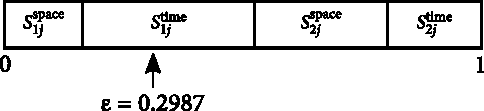
\includegraphics{figures/hidden_variables/random_choice.pdf}
    \caption{Probabilistically choosing a transition. Top: Probability flows between states in a time interval according to the three matrices of unconditional probabilities $P^\up{stay}$, $P^\up{space}$, and $P^\up{time}$ in such a way that one total unit of probability is routed from states at the initial time to states at the final time consistent with the populations resulting from quantum mechanical evolution in that timestep. Centre: The hidden variable transitions according to the corresponding conditional probabilities, which are elements of the matrices $S^\up{stay}$, $S^\up{space}$, and $S^\up{time}$. Here the hidden variable is in state $1$ and we are choosing whether it will remain in that state or if it will transition to state $2$ or $3$, and whether it transitions via a spatial or temporal non-adiabatic transition. Bottom: All the probabilities for what may happen to the hidden variable in a timestep sum to one, so an array of the cumulative probabilities can be constructed, and a random number drawn from the range $[0,1]$. The index of the smallest element of the array of cumulative sums that the random number is smaller than corresponds to the event to occur. In the above diagrammatic example, the result of the random draw is that the hidden variable is to transition to state $2$ via a spatially induced non-adiabatic transition.}\label{fig:random_choice}
\end{figure}

\subsubsection{Framing fewest-switches as a hidden-variable theory}

Tully's fewest-switches algorithm allows one to compute transition probabilities for a hidden variable given the Hamiltonian, the state amplitudes, and a small interval of time. Does this satisfy Aaronson's definition of a hidden-variable theory (Section~\ref{sec:hidden_variable_theories})? As written, not quite, since it requires the Hamiltonian rather than the unitary that describes state vector evolution over a particular time interval. However it is simple to reconcile the two sets of requirements. Given that the interval of time is small, the unitary describing evolution in the local basis can be linked to the effective Hamiltonian in~\eqref{eq:Tully_adiabatic_eff} via
\begin{align}
\hat U(t+\dd t, t) = \ee^{-\frac\ii\hbar\hat H_\up{eff}(\vec r, t)\,\dd t},
\end{align}
where
\begin{align}
\hat H_\up{eff} = \hat V(\vec r, t)
  - \ii\hbar\hat U_H(\vec r, t)\dv{t}U^\dagger_H(\vec r, t)
\end{align}
is the effective Hamiltonian in the adiabatic picture for $\hat H$, the matrix representation of which can be extracted from the matrix representation of $\hat U(t+\dd t, t)$ as
\begin{align}
H_\up{eff}(\vec r, t)\,\dd t &= \ii\hbar\Log U(t+\dd t, t)\\
&\approx \ii\hbar\left(\mathbb{I} -  U(t+\dd t, t)\right)
\end{align}
where $\Log$ is the principal value of the complex matrix logarithm.

Since only the matrix $H_\up{eff}(\vec r, t)\,\dd t$ is required to compute transition probabilities according to~\eqref{eq:fewest_switches_Heff}, and not its component terms,\footnote{Though we do need its component terms if we wish to distinguish between spatially vs.\ temporally induced transitions as in Section~\ref{sec:fewest_switches}.} specifying the initial state vector and unitary for an interval of time evolution (both in the local basis) is a sufficient input to be able to compute transition probabilities using Tully's fewest-switches algorithm. Writing the resulting matrix of probabilities in terms of $U$ gives:
\begin{align}
P_{ij} = \begin{cases}
\max\left\{0, 2\re\left(c_i^*(t)U_{ij}(t + \dd t, t)c_j(t)\right)\right\} & i \neq j\\
\abs{c_i(t)}^2 - \sum_{j\neq i} P_{ij} & i = j
\end{cases}.
\end{align}
The corresponding stochastic matrix $S$ can then be obtained by scaling the columns of $P$ by the state populations as in~\eqref{eq:P_matrix_def}. Tully's fewest-switches algorithm thus satisfies Aaronson's definition of a hidden-variable theory provided that the time interval is small. The low computational complexity of computing probabilities via fewest-switches is somewhat remarkable. There is no matrix scaling, no matrix permanents, or any other large computational expense.

Expressed in Python, Tully's fewest-switches can be computed very simply as shown below, though this calculation is only first-order accurate in the time interval corresponding to the unitaries.

\python{code_listings/tully_fewest_switches.py}

It is not clear how many of Aaronson's axioms are satisfied by fewest-switches, but the dependence of its probabilities on the actual coupling strengths between states via the non-adiabatic Hamiltonian (and vanishing probabilities when those coupling strengths are zero) is encouraging, and ensures that its behaviour is free of the pathology of the product theory. Furthermore, the form of fewest-switches when framed in terms of the unitary for the given time interval is quite similar to that of Schr\"odinger theory. In Schr\"odinger theory one takes the absolute value of elements of $U$ and then applies row and column scalings. In fewest-switches one applies row and column scalings (explicitly given as $c_i^*(t)$ and $c_j(t)$, along with a factor of $2$), then takes the real part of the result and clips it to zero from below. The two methods are not identical, but the similarity is striking.

\subsection{Velocity correction and classically disallowed transitions}\label{sec:velocity_correction}

When a transition of the hidden variable occurs due to a spatial non-adiabatic transition, the kinetic energy of the atom must be adjusted to conserve overall energy. The force on an atom during a transition from the $j^\up{th}$ state to the $i^\up{th}$ state due to the spatial non-adiabatic coupling term in the effective Hamiltonian is in the direction of the non-adiabatic coupling vector~\cite{doi:10.1146/annurev-physchem-040215-112245}
\begin{align}\label{eq:non_adiabatic_coupling_vector}
\vec d_{ij}(\vec r, t) &= \matrixel{\chi_i(\vec r, t)}{\nabla}{\chi_j(\vec r, t)}\\
&= \left(U_H(\vec r, t)\nabla U_H^\dagger(\vec r, t)\right)_{ij}
\end{align}
where $U_H(\vec r, t)$ is the matrix representation, in any (spatially and temporally fixed) basis, of the unitary that takes state vectors into the basis in which $\hat H(\vec r, t)$ is diagonal, defined by~\eqref{eq:U_H_definition}. To conserve energy, the squared component of an atom's velocity in this direction must change by an amount:
\begin{align}\label{eq:delta_v_squared}
\upDelta v_{ij}^2 = \frac2m\left(V_j(\vec r, t) - V_i(\vec r, t)\right),
\end{align}
where $V_i(\vec r, t)$ is the adiabatic potential comprising the $i^\up{th}$ spatially and/or temporally varying eigenvalue of $\hat H(\vec r, t)$. However, it is possible that a change of this size can leave an atom with a negative kinetic energy. Whilst this is quantum-mechanically permissible, it is forbidden classically, and so we simply disallow such transitions, defining a modified matrix of unconditional transition probabilities $\tilde P^\up{space}$ that sets the probability of the disallowed transitions to zero:
\begin{align}\label{eq:tilde_P_space}
\tilde P^\up{space}_{ij} =
\begin{cases}
P^\up{space}_{ij} & \upDelta v_{ij}^2 + \abs{\vec v\cdot\hat{\vec d}_{ij}}^2 \geq 0 \\
0 & \upDelta v_{ij}^2 + \abs{\vec v\cdot\hat{\vec d}_{ij}}^2 < 0
\end{cases}
\end{align}
where $\hat{\vec d}_{ij} = \hat{\vec d}_{ij}(\vec r, t)$ is the unit vector in the direction of $\vec d_{ij}(\vec r, t)$.\footnote{The surface-hopping literature calls these classically disallowed transitions \emph{frustrated} transitions. Prior to encountering the surface-hopping literature, my method of conserving energy was identical to this (for the case of time-independent potentials), with the exception that I did not know what direction the velocity kick ought to be in, limiting my method to one spatial dimension only. There is much interest in alternate methods of energy conservation in chemical physics, however so far this has been outside of my interest in these methods for simulating cold atoms.}

The diagonal matrix for the probabilities of remaining in each state must be adjusted similarly to absorb the probability discarded this way:
\begin{align}
\tilde P^\up{stay}_{ii} = 
\abs{c_i(t)}^2 - \sum_{j\neq i}\left(\tilde P^\up{space}_{ij} + P^\up{time}_{ij}\right)
\end{align}
The corresponding matrices of conditional probabilities for the hidden variable transitioning, given that it is already in the $j^\up{th}$ state, are
\begin{align}\label{eq:tilde_S_space}
\tilde S^\up{space}_{ij} &= \frac1{\abs{c_j(t)}^2} \tilde P^\up{space}_{ij},\\
\tilde S^\up{stay}_{ij} &= \frac1{\abs{c_j(t)}^2} \tilde P^\up{stay}_{ij},
\end{align}
Of course, when making probabilistic transitions of the hidden variable, the originating state is known and so only one column of any of the above matrices is used at a time, so the full matrices $\tilde P^\up{space}$, $\tilde P^\up{time}$, $\tilde S^\up{space}$, and $\tilde S^\up{time}$ do not need to be computed at each timestep.

In the case that a transition of the hidden variable does occur to the $i^\up{th}$ from the $j^\up{th}$ state due to a spatial non-adiabatic coupling, the velocity kick to be applied to the classical velocity vector in order to conserve energy is
\begin{align}\label{eq:velocity_jump}
\upDelta \vec v_{ij} = \left[\sgn(\vec v\cdot \hat{\vec d}_{ij})
\sqrt{(\vec v\cdot \hat{\vec d}_{ij})^2 + \frac2m\left(V_i(\vec r, t) - V_j(\vec r, t)\right)} - (\vec v\cdot \hat{\vec d}_{ij}).
\right]\hat{\vec d}_{ij}
\end{align}   

\section{Decoherence}\label{sec:decoherence}

In the context of the hidden-variable semiclassical/surface-hopping method, \emph{decoherence} refers to the fact that, due to positional separation of different internal states of the atom, those internal states transition from being a coherent superposition into a statistical mixture. For example, in the Stern--Gerlach experiment, a spin may be initially a coherent superposition of spin-up and spin-down, but by the time the two components separate, the superposition is no longer a coherent one. The spin is either up (and the atom off to one side of the screen) or down (and the atom over the other side of the screen). At this point, no interference between the two internal states is observable, as they are not co-located in space. The motional degree of freedom has played the role of an environment, and, having become entangled with the spin of the atom, decohered the spin state. Recoherence can occur if the two wavepackets are brought back together again to have well overlapping positions and velocities, but this is difficult to achieve even intentionally,\footnote{The problem of getting the wavepackets back together again has been coined the `Humpty-Dumpty problem'~\cite{Schwinger1988, doi:10.1063/1.459170} and has made magnetic separation impractical for large-momentum atom interferometry~\cite{machluf_coherent_2013}, and methods such as the use of Bragg pulses~\cite{PhysRevLett.66.2693, PhysRevLett.75.2633} are needed to create large momentum differences between wavepackets without having them more slowly traverse the intermediate regions of momentum space where they might accumulate coherence-destroying phase noise.} let alone by accident, 

Decoherence was not part of Tully's original surface-hopping model~\cite{doi:10.1063/1.459170}, such that if used to simulate the Stern--Gerlach experiment, two spots would result on the screen, but both spots would comprise a coherent $50:50$ superposition of spin-up and spin-down, rather than one being up and one being down. Some decoherence is necessary to include in a hidden-variable semiclassical/surface-hopping model in order to avoid this unphysical outcome, and furthermore, to obtain correct transition probabilities in the case that the atom undergoes multiple periods of local spin transitions (as being in a $50:50$ superposition represents entirely different initial conditions for a Majorana spin flip than being in a single spin state).

Our approach to modelling decoherence requires some assumptions about the motional states of the atom and how they evolve in time. We therefore construct wavepackets that are as classical as we can make them, being as localised in position and velocity space as they can be. For this we use Gaussian wavepackets of width equal to the thermal de~Broglie wavelength $\sigma = \lambda_\up{th} = h/\sqrt{2\pi m k_\up{B} T}$, evolving without dispersion, with their centre-of-mass position and velocity evolving classically according to the adiabatic potential experienced by the eigenstate to which each motional state corresponds.

In Section~\ref{sec:backaction} I show the general mechanism by which the divergence of trajectories decoheres internal states of an atom, and specifically how this manifests as a decrease in the amplitude of every other state when one imposes the adiabatic trajectory corresponding to a specific internal state. I then show in Sections~\ref{sec:zeno_effect} and~\ref{sec:continuous_projection} why na\"ively projecting the wavefunction onto a single trajectory at all times yields nonsensical results, and then in Subsections~\ref{sec:markovian_decoherence} and~\ref{sec:spawned_trajectories} I present two remedies for how to approximately include decoherence in spite of this. 

The development of the second of these remedies brought to light a possibility I hadn't considered before, regarding the form of the `classical' state that the total wavefunction is projected onto at each timestep. Namely, that it makes some sense for this to be a Dirac delta instead of a Gaussian wavepacket. In light of this, in Section~\ref{sec:dirac_deltas} I present an alternative view of what it means to `follow' a wavepacket, and expressions for the decoherence rates of the two methods under this alternate assumption. I argue why this is appealing and why it resolves some issues that are present when projecting onto a Gaussian wavepacket.

\subsection{Back-action of position measurement on internal state}\label{sec:backaction}

Consider an atom in a state $\ket{\Psi(t)}$, which is an arbitrary superposition of internal basis states $\ket{\chi_i}$ and motional basis states $\ket{\vec r}$: 
\begin{align}
\ket{\Psi(t)} = \int \sum_i \psi_i(\vec r, t) \ket{\chi_i}\otimes\ket{\vec r} \dd\vec r,
\end{align}
where normalisation requires that
\begin{align}
\int \sum_i \abs{\psi_i(\vec r, t)}^2 \dd\vec r = 1.
\end{align}
Recognising $\psi_i(\vec r, t)$ as the $i^\up{th}$ component of a multi-component wavefunction, we define (up to an arbitrary phase factor) a normalised wavefunction $\phi_i(\vec r, t)$ and corresponding motional state vector $\ket{\phi_i(t)}$ and its coefficient $c_i(t)$ for each internal state:
\begin{align}\label{eq:product_state_vector}
c_i(t)\phi_i(\vec r, t) &\equiv \psi_i(\vec r, t) \\
\ket{\phi_i(t)} &\equiv \int \phi_i(\vec r, t)\ket{\vec r}\dd \vec r
\end{align}
such that $\int\abs{\phi_i(\vec r, t)}^2\dd \vec r = 1$. This allows us to write our arbitrary state vector as a sum over the internal basis only:
\begin{align}
\ket{\Psi(t)} = \sum_i c_i(t) \ket{\chi_i}\otimes\ket{\phi_i(t)},
\end{align}
where the spatial state vectors $\{\ket{\phi_i(t)}\}$ are not necessarily orthogonal. To see that spatial separation of the different components leads to decoherence of the internal states, consider the pure density operator corresponding to $\ket{\Psi(t)}$:
\begin{align}
\hat\rho(t) = \ketbra{\Psi(t)}{\Psi(t)} = \sum_{ij}
c_i(t) c_j^*(t)\ketbra{\chi_i(t)}{\chi_j(t)}\otimes\ketbra{\phi_i(t)}{\phi_j(t)},
\end{align}
which we can write in the $\{\ket{\chi_i}\otimes\ket{\vec r}\} \equiv \{\ket{\chi_i\ \vec r}\} $ basis, resulting in matrix elements
\begin{align}
\rho_{ij}(t, \vec r, \vec r^\prime) &= \matrixel{\chi_i\ \vec r}{\rho(t)}{\chi_j\ \vec r^\prime},\\
&= \psi_i(\vec r, t)\psi_j^*(\vec r^\prime, t),\\
&= c_i(t) c^*_j(t) \phi_i(\vec r, t) \phi_j^*(\vec r^\prime, t).
\end{align}
A partial trace~\cite{schlosshauer_decoherence:_2007} over the motional degree of freedom results in a reduced density operator describing the measurement statistics of the internal degree of freedom only:
\begin{align}
\hat\rho^\up{red}(t) &= \int\matrixel{\vec r}{\hat \rho(t) \hat {\vec r}}{\vec r}\dd \vec r\\
\Rightarrow \rho^\up{red}_{ij}(t) &= \int\rho_{ij}(t, \vec r, \vec r^\prime)\delta(\vec r - \vec r^\prime)\dd \vec r\\
&= c_i(t) c_j^*(t)\int\phi_i(\vec r, t)\phi_j^*(\vec r, t)\dd \vec r\\
&= c_i(t) c_j^*(t)\braket{\phi_j(t)}{\phi_i(t)}\label{eq:rho_with_decoherence}.
\end{align}
The off diagonals of the density matrix $\rho^\up{red}_{ij}(t)$, representing the coherences of the internal states, are reduced by a factor $\braket{\phi_j(t)}{\phi_i(t)}$, which will be unity only for pairs of motional state vectors that are identical. We therefore see that spatial separation of the wavefunctions corresponding to different internal states leads to decoherence of the internal states, and we define the decoherence factor
\begin{align}\label{eq:decoherence_factor_definition}
R_{ij}(t) = \braket{\phi_i(t)}{\phi_j(t)},
\end{align}
such that~\eqref{eq:rho_with_decoherence} reads
\begin{align}
\rho^\up{red}_{ij}(t) &= c_i(t) c_j^*(t) R_{ij}^*(t) \nonumber\\
& = c_i(t) c_j^*(t) R_{ji}(t).
\end{align}
This same decoherence factor appears when---instead of integrating over all positions---we project the total state vector onto a single motional state corresponding to a classical trajectory, which is how we impose classicality on the motional degree of freedom in our model. The effect of decoherence when `following' a specific motional state through space in this way is to reduce the amplitudes of all other states not being followed, by the decoherence factor between that state and the one being followed, as shown schematically in~\figref{fig:HVSC_schematic}.

To obtain an explicit form for the decoherence factor, we need to impose an ansatz for the motional states $\{\ket{\phi_i(t)}\}$. We take each motional state $\ket{\phi_i(t)}$ to be a Gaussian wavepacket propagating---without dispersion---with centre-of-mass motion evolving classically according to the adiabatic potential $V_i(\vec r, t)$ experienced by the local eigenstate $\ket{\chi_i}$. Thus the wavefunctions of these motional states are
\begin{align}
\braket{\vec r}{\phi_i(t)} &= \phi_i(\vec r, t) = A\exp\left[-\frac{\abs{\vec r - \vec r_i(t)}^2}{4\sigma^2} + \ii \frac m\hbar \vec v_i(t)\cdot (\vec r - \vec r_i(t))\right],
\end{align}
Where $\vec r_{ij}(t) = \vec r_i(t) - \vec r_j(t)$ and $\vec k_{ij}(t) = \frac m\hbar \left(\vec v_i(t) - \vec v_j(t)\right)$ are the mean displacement and relative wavevector of the pair of wavepackets, $A$ is a real normalisation constant,\footnote{The overall phase is determined by the offset $\vec r - \vec r_i(t)$ in the second term in the exponent, and is chosen such that $\phi_i(\vec r, t)$ is real at $\vec r=\vec r_i$, which ensures that $\braket{\phi_i(t)}{\phi_j(t)}$ has a phase depending only on the mean displacement of the two wavepackets rather than their distance from some arbitrary origin. This prevents an additional arbitrary phase at each timestep of the model, which would not affect the dynamics but is unappealing.} and where the centre-of-mass position and velocity of each wavepacket evolve classically according to
\begin{align}\label{eq:classical_const_a_first}
\dv{t} \vec r_i(t) &= \vec v_i(t)\\
\dv{t} \vec v_i(t) &= -\frac1m\nabla V_i(\vec r_i, t).
\label{eq:classical_const_a_second}
\end{align}
This yields the decoherence factor:
\begin{align}\label{eq:decoherence_factor}
R_{ij}(t) = \exp\left[-\left(\frac1{8\sigma^2}\abs{\vec r_{ij}}^2
+ \frac\ii 2 \vec r_{ij}(t) \cdot \vec k_{ij}(t) + \frac{\sigma^2}{2} \abs{\vec k_{ij}(t)}^2
\right)\right].
\end{align}
As expected, $R_{ij}(t)$ is equal to unity when the two wavepackets have identical positions and velocities, and decays to zero for increasing relative position and velocity. 

If the two motional states being considered are identical at $t=0$ and have constant relative acceleration $\vec a_{ij}$, then we have
\begin{align}
\vec r_{ij}(t) = \frac12\vec a_{ij} t^2;\\
\vec k_{ij}(t) = \frac m \hbar \vec a_{ij} t,
\end{align}
and~\eqref{eq:decoherence_factor} reduces to
\begin{align}\label{eq:const_a_decoherence_factor}
R_{ij}(t) = \exp\left[-\frac {\abs{\vec a_{ij}}^2} 2 \left(\frac1 {16\sigma^2}t^4 + \ii\frac m{2\hbar}t^3 + \frac{m^2\sigma^2}{\hbar^2} t^2 \right)\right].
\end{align}
We will use this expression in Sections~\ref{sec:markovian_decoherence} in order to derive approximate decoherence rates under the assumption of uniform relative acceleration.

We are now placed to precisely define what we mean by `following' a trajectory.
Returning to our arbitrary state vector~\eqref{eq:product_state_vector}, we define (ignoring normalisation) the projected state vector
\begin{align}\label{eq:R_projection}
\ket{\tilde \Psi(t)} = \hat R(t)\ket{\Psi(t)},
\end{align}
where $\hat R(t) = \hat 1 \otimes \ketbra{\phi_\eta(t)}{\phi_\eta(t)}$, that results from the projection of $\ket{\Psi(t)}$ onto the specific motional state $\ket{\phi_\eta(t)}$ corresponding to the hidden variable $\eta(t)$. This gives (neglecting normalisation) the state vector one would observe conditional on the particle being in that specific motional state at that specific time:
\begin{align}
\ket{\tilde \Psi(t)} &= \hat R(t) \ket{\Psi(t)}\\
&= \sum_i\braket{\phi_\eta(t)}{\phi_i(t)}c_i(t)\ket{\chi_i}\otimes\ket{\phi_\eta(t)}\\
&= \sum_i\tilde c_i(t)\ket{\chi_i}\otimes\ket{\phi_\eta(t)}\\
&= \ket{\tilde \chi(t)}\otimes\ket{\phi_\eta(t)},
\end{align}
where we have defined $\tilde c_i(t) = \braket{\phi_\eta(t)}{\phi_i(t)}c_i(t)$ and $\ket{\tilde \chi(t)} = \sum_i \tilde c_i(t)\ket{\chi_i}$. We recognise $\braket{\phi_\eta(t)}{\phi_i(t)}$ as the decoherence factor $R_{\eta i}(t)$ defined in~\eqref{eq:decoherence_factor_definition}, and can immediately see that the effect of such projection is to reduce the amplitude of all other states ($i\neq\eta$) by this factor.

\subsection{Continuous projection}\label{sec:continuous_projection}
We now consider the following protocol: project the state vector at time $t$ as per~\eqref{eq:R_projection}, evolve the resulting state vector to $t+dt$ under the action of a projected Hamiltonian, and repeat. In Section~\ref{sec:zeno_effect} I show that this continuous projection yields unphysical decoherence rates, such that the following derivation will need to be modified in order to usefully model decoherence. Nonetheless this establishes the form of the back-action caused by projections in terms of a decoherence rate, and connects this rate to the decoherence factor~\eqref{eq:decoherence_factor_definition}. The result is salvageable, and in Sections~\ref{sec:markovian_decoherence} and~\ref{sec:spawned_trajectories} I present two methods of computing physically meaningful decoherence rates for use in the resulting equation of motion for the projected state vector.

The state vector evolved to time $t+\dd t$ and re-projected with $\hat R(t + \dd t)$ is
\begin{align}\label{eq:second_proj}
\ket{\tilde \Psi(t + \dd t)} &= 
\hat R(t + \dd t)
\sum_i
\left[\tilde c_i(t) - \frac\ii\hbar\sum_j H_{ij}(t)\tilde c_j(t)\dd t\right]
\ket{\chi_i}\otimes\ket{\phi_i(t + \dd t)},
\end{align}
where $H_{ij}(t) = \matrixel{\chi_i}{\hat H_{\eta}(t)}{\chi_j} = \matrixel{\chi_i\ \phi_\eta(t)}{\hat H(t)}{\chi_j\ \phi_\eta(t)}$ are the matrix elements of the projected Hamiltonian $\hat H_\eta(t)$ dictating the dynamics of the internal state, given the imposed motional state $\ket{\phi_\eta}$ and the total Hamiltonian $\hat H(t)$ of the system. Note that because of the previous projection already performed, all motional states $\ket{\phi_i(t)}$ were `reset' to be equal to $\ket{\phi_\eta(t)}$ at time $t$, and therefore the evolved motional state $\ket{\phi_i(t + \dd t)}$ represents the evolution of the motional state corresponding to the $i^\up{th}$ internal state over an interval $\dd t$, starting with the initial condition $\ket{\phi_\eta(t)}$. Accordingly, both motional states will still be approximately equal after this short evolution, allowing us to write
\begin{align}
\braket{\phi_\eta(t + \dd t)}{\phi_i(t + \dd t)} &= \braket{\phi_\eta(t)}{\phi_i(t)} + \dv{t}\braket{\phi_\eta(t)}{\phi_i(t)}\dd t\\
& = 1 + \dv{R_{\eta i}(t)}{t}.
\end{align}
Using this fact in applying the projection in~\eqref{eq:second_proj} yields a product state once more:
\begin{align}
\ket{\tilde \Psi(t + \dd t)} &= 
\sum_i
\left(1 + \dv{r_{\eta i}(t)}{t}\right)
\left[\tilde c_i(t) - \frac{\ii}\hbar\sum_j H_{ij}(t) \tilde c_j(t)\dd t\right]
\ket{\chi_i}\otimes\ket{\phi_\eta(t + \dd t)}\\
\Rightarrow \ket{\tilde \chi(t + \dd t)} &= \sum_i
\left(1 + \dv{r_{\eta i}(t)}{t}\right)
\left[\tilde c_i(t) - \frac{\ii}\hbar\sum_j H_{ij}(t) \tilde c_j(t)\dd t\right]
\ket{\chi_i}
\end{align}
which we can solve for $\frac1{\dd t}\left(\ket{\tilde \chi(t + \dd t)} - \ket{\tilde \chi(t)}\right)$ to obtain a differential equation for $\ket{\tilde \chi(t)}$:
\begin{align}
\dv{t} \ket{\tilde \chi(t)} =
\left[-\frac\ii\hbar\hat H_\eta(t) - \hat\Gamma_\eta(t)\right]\ket{\tilde\chi(t)},
\end{align}
where $\hat\Gamma_\eta(t)$ is a diagonal operator in the $\{\ket{\chi_i}\}$ basis with elements
\begin{align}
(\Gamma_\eta(t))_{ii} = \gamma_{\eta i}(t) = -\dv{R_{\eta i}(t)}{t} = -\dv{t} \braket{\phi_\eta(t)}{\phi_i(t)},
\end{align}
where we have defined $\gamma_{ij}(t) = -\dv{R_{ij}(t)}{t}$. The diagonals of $\hat \Gamma_\eta(t)$ in the adiabatic basis are \emph{decoherence rates}, and cause exponential damping of all internal states other than the $\ket{\chi_\eta}$ state. The damping rates increase with the rate at which the given internal state diverges from $\ket{\phi_\eta(t)}$.

\subsection{The quantum Zeno effect}\label{sec:zeno_effect}

But now we arrive at a problem. Because all the motional states are reset to be equal to $\ket{\phi_\eta(t)}$ at each timestep as in~\eqref{eq:second_proj}, the relative position and wavevector of the two wavepackets are zero at all times, and so our decoherence rates are:
\begin{align}
\gamma_{ij} &= -\left[\dv{R_{ij}(t)}{t}\right]_{
\stackon[1pt]
{$\scriptscriptstyle\, \vec v_{ij} = 0$}
{$\scriptscriptstyle\, \vec k_{ij} = 0$}
}\\
&= -\left[
\pdv{R_{ij}(t)}{\vec r_{ij}}\cdot \dv{\vec r_{ij}(t)}{t} + 
\pdv{R_{ij}(t)}{\vec k_{ij}}\cdot \dv{\vec k_{ij}(t)}{t}\right]_{
\stackon[1pt]
{$\scriptscriptstyle\, \vec v_{ij} = 0$}
{$\scriptscriptstyle\, \vec k_{ij} = 0$}
}\\
&= \left[
\left(
\frac{\vec r_{ij}}{4\sigma^2} + \frac\ii2\vec k_{ij}
\right)R_{ij}(t)\cdot\dv{\vec r_{ij}(t)}{t}
+ \left(
\sigma^2\vec k_{ij} + \frac\ii2\vec r_{ij}
\right)R_{ij}(t)\cdot\dv{\vec k_{ij}(t)}{t}
\right]_{
\stackon[1pt]
{$\scriptscriptstyle\, \vec v_{ij} = 0$}
{$\scriptscriptstyle\, \vec k_{ij} = 0$}
}\\
&= 0.
\end{align}
Every decoherence rate is zero. What is going on? The answer is the quantum Zeno effect~\cite{PhysRevA.41.2295, doi:10.1063/1.523304}, which is the name given to the fact that, in the limit of infinitely frequent measurements of whether quantum evolution has occurred, the back-action of the measurement has the effect of preventing the evolution from occurring at all. In our case, the fact that we are constantly projecting onto the followed motional state causes the amplitude flows to the other motional states to be exactly zero. A sufficiently closely watched quantum pot never boils, and a sufficiently closely watched Schr\"odinger's cat never may never be poisoned~\cite{doi:10.1063/1.523304}:
\begin{quote}
In view of
the Zeno's paradox formulated above, should we conclude
that the particle will never decay? Will the cat
escape the cruel death awaiting it, against which it has
no defense, provided its vital signs are constantly
watched with loving care? 
\end{quote}
The appearance of the quantum Zeno effect ought to be a reminder that the assumption of infinitely frequent projective measurements is unphysical. In our case it certainly is---we have merely imagined a hypothetical measurement device collapsing our position states because we don't want to simulate them, not because any such measurement device actually exists. Nonetheless the internal states of the atom \emph{do} decohere even in the absence of measurement (and there is eventual measurement when the atoms collide with other atoms or otherwise interact with anything in a position-dependent way), and we wish to model the approximate effect of this, if possible with a differential equation that does not require us to simulate all the quantum details of the motional degree of freedom.

Note that if the decoherence factor had the form of exponential decay:
\begin{align}
R^\up{Markov}_{ij}(t) = \ee^{-\gamma_{ij} t}, 
\end{align}
then the decoherence rate would be the constant $\gamma_{ij}$, and not zero. This is the case for Markovian decoherence~\cite{schlosshauer_decoherence:_2007}, which is when the environment has no memory of its past interaction with the system. The memory in our case is due to the wavepackets accelerating away from each other, starting from zero relative position and velocity at each timestep---the relative position and velocity comprise a memory of the past interaction, which we are erasing each time we reproject.

The lack of an environmental memory is only ever approximately true, and no decoherence factors in nature have the form of a decaying exponential at all times. At small enough times the overlap between two states can only move away from unity quadratically owing to unitary evolution on account of the Schr\"odinger equation, guaranteeing an initial time derivative of zero for all physical decoherence factors. However in many systems of interest, the specifics of the interaction with the system are quickly forgotten by the environmental states, and the decoherence factor does approach a decaying exponential~\cite{0034-4885-41-4-003}. This is the case, for example, for spontaneous photon emission by atoms, which one can consider a measurement effect in which the electromagnetic field is being regularly measured by the environment in the photon number basis~\cite{1355-5111-8-1-015, Molmer:93, RevModPhys.70.101}. In the various quantum trajectories methods used to simulate atoms in the presence of spontaneous emission, if one assumes that the measurements are projective, one must simply assume that the frequent measurements take place at large enough timescales that the decoherence factor is in the exponential decay regime, provided that this is much smaller than other dynamical timescales, which is true for spontaneous emission~\cite{RevModPhys.70.101}. The measurement interval assumed ``should be large enough to allow the photons to get away from the atom"~\cite{2003LNP...622..233H}. This can be recast as a continuous \emph{weak} measurement, rather than infrequent projective measurements~\cite{doi:10.1080/00107510601101934, RevModPhys.70.101}, which is more physically realistic than the assumption of projective measurements at somewhat arbitrarily chosen intervals, but results in the same differential equations.

A decoherence factor that has the form of a decaying exponential implies that any chosen measurement interval results in the same fractional reduction in state amplitudes, since the differential equation $\dv{\tilde c_{i}(t)}{t} = -\gamma \tilde c_i(t)$ has the solution $\tilde c(t) = \ee^{-\gamma t} \tilde c(0)$, that is, repeated consideration of only the first part of the decoherence factor ends up tracing out the whole decoherence curve over time.

How can we replicate something like this for our separating wavepackets? Here I present two approaches. The first, described in Section~\ref{sec:markovian_decoherence}, is to gloss over as many of the details of the wavepacket separation as possible and replace the decoherence factor with an exponential one, describing the wavepackets separating on approximately the correct timescale. This is crude, but better than no decoherence at all. The second, described in Section~\ref{sec:spawned_trajectories}, is to introduce a minimal memory of the separation of wavepackets. In this approach, one (but only one) trajectory is simulated for the motional state corresponding to each internal state. Whenever there is population transfer from the main trajectory to another state, the trajectory corresponding to the other state is replaced with a weighted average of its existing position and velocity with the position and (adjusted for energy conservation) velocity of the main trajectory. These \emph{auxiliary trajectories} are used to compute a dynamic decoherence rate that traces out a more correct decoherence curve as the wavepackets separate.

\subsection{Approximate Markovian decoherence}\label{sec:markovian_decoherence}

A crude way to include decoherence is just to approximate $R_{\eta i}(t)$---for the case of constant acceleration in~\eqref{eq:const_a_decoherence_factor}---as a decaying exponential with roughly the right decay constant. This is crude because $R_{\eta i}(t)$ does not look much like a decaying exponential (see~\figref{fig:decoherence_factor_example}). In the limit of large $t$, its functional form is $\ee^{-t^4}$, not the exponential decay required to treat the decoherence as Markovian at any timescale.

\begin{figure}[t]
    \centerfloat
    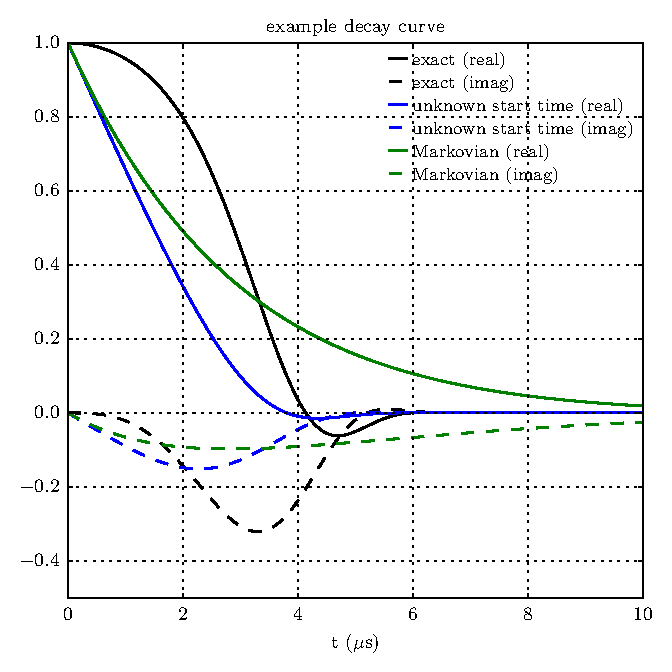
\includegraphics{figures/hidden_variables/decoherence_factor_example.pdf}
    \caption{Example decoherence factor~\eqref{eq:const_a_decoherence_factor} as a function of time for an experimentally realistic parameters. Plotted in black is the exact decoherence factor $R_{ij}(t)$ given by ~\eqref{eq:const_a_decoherence_factor} between two adjacent ($\upDelta m_F = \pm 1$) Zeeman sublevels of the $F=1$ ground state of $^{87}$Rb, assuming constant relative acceleration due to a magnetic field gradient of $250\unit{G\,cm}^{-1}$ and a Gaussian wavepacket width $\sigma=\lambda_\up{th} = 2.6\unit{\mu m}$, corresponding to the thermal wavelength $\lambda_\up{th} = h/\sqrt{2\pi m k_\up{B} T}$ at $T=53\unit{\upmu K}$. Shown in blue is the `time-ignorant' decoherence factor described in text. In green is the Markovian approximation to the exact decoherence factor, obtained by extracting a decay constant from the gradient of the time-ignorant decoherence factor at $t=0$. As can be seen, whilst no decaying exponential is a particularly good fit to the exact decoherence factor, our Markovian approximation is as good as can be expected, decaying to zero over approximately the correct timescale.}
    \label{fig:decoherence_factor_example}
\end{figure}

To nonetheless find an approximate Markovian decoherence rate, we first construct a `time ignorant' version $\tilde R_{ij}(t)$ of the decoherence factor $R_{ij}(t)$ given in~\eqref{eq:const_a_decoherence_factor} that answers the question ``What is the expected value of $R_{ij}(t)$ at all times $t > 0$ if I don't know how long before $t=0$ the two wavepackets began separating?" 

We can then take the derivative of this time-ignorant decoherence factor at $t=0$ to use as an approximate Markovian decoherence rate $\gamma_{ij}^\up{Markov}$. Whilst extremely approximate, this method of including decoherence is nonetheless an improvement over the Ehrenfest method (which has no decoherence), and over Tully's original fewest-hops surface-hopping method~\cite{doi:10.1063/1.459170}, which also lacked any decoherence. Others~\cite{doi:10.1063/1.4733675, doi:10.1063/1.1468887, doi:10.1063/1.470177} have since developed various methods to induce approximate damping of states to achieve a similar outcome, including the approximation of an exponential decoherence factor~\cite{doi:10.1063/1.4733675}, though my development of this method was independent.

Proceeding, we define the time-ignorant decoherence factor $\tilde R_{ij}(t)$ as the average of all decoherence factors one would obtain if the two wavepackets began separating at some point in time before $t=0$:
\begin{align}
\tilde R_{ij}(t) &= A\int_{-\infty}^0\braket{\phi_i(t-t^\prime)}{\phi_j(t - t^\prime)} \,\dd t^\prime\\
&= A\int_{-\infty}^0 R_{ij}(t-t^\prime) \,\dd t^\prime.
\end{align}
Here, $A$ is a normalisation constant such that $\tilde R_{ij}(0) = 1$, and where we take that $\ket{\phi_i(0)} = \ket{\phi_j(0)}$ with each thereafter evolving according to the classical motion of their centre of mass with constant relative acceleration as in~\eqref{eq:classical_const_a_first} and~\eqref{eq:classical_const_a_second} such that the $R_{ij}(t)$ above has the form of~\eqref{eq:const_a_decoherence_factor}.

Our time-ignorant decoherence rate is then the (negative of the) derivative of $\tilde R_{ij}(t)$ at $t=0$:
\begin{align}
\gamma_{ij}^\up{Markov} = -\left[\dv{\tilde R_{ij}(t)}{t}\right]_{t=0} = -\frac{\left[\dv{t}\int_{-\infty}^0 R_{ij}(t-t^\prime) \,\dd t^\prime\right]_{t=0} }
{\left[\int_{-\infty}^0 R_{ij}(t-t^\prime) \,\dd t^\prime\right]_{t=0}}.
\end{align}
Moving the derivative inside the integral, noting that $\dv{R_{ij}(t - t^\prime)}{t} = \dv{R_{ij}(t - t^\prime)}{(t - t^\prime)}$ and setting $t = 0$, we get:
\begin{align}
\gamma_{ij}^\up{Markov} &= -\frac
{\int_{-\infty}^0 R_{ij}^\prime(-t^\prime) \,\dd t^\prime}
{\int_{-\infty}^0 R_{ij}(-t^\prime) \,\dd t^\prime}\\
&= -\frac
{\int_0^\infty R_{ij}^\prime(t^\prime) \,\dd t^\prime}
{\int_0^\infty R_{ij}(t^\prime) \,\dd t^\prime}
\end{align}
where $R_{ij}^\prime$ is the derivative of $R_{ij}$ with respect to its argument. By the fundamental theorem of calculus the numerator is $-1$, since $R_{ij}(t)$ decreases from unity at $t=0$ to zero as $t$ goes to infinity, leaving us with:

\begin{align}\label{eq:gamma_integral}
\frac1{\gamma_{ij}^\up{Markov}} &= 
  \int_0^\infty R_{ij}(t^\prime) \,\dd t^\prime\\
&= \int_0^\infty \exp\left[-\left(\frac1{8\sigma^2}\abs{\vec r_{ij}}^2
+ \frac\ii 2 \vec r_{ij}(t^\prime) \cdot \vec k_{ij}(t^\prime) + \frac{\sigma^2}{2} \abs{\vec k_{ij}(t^\prime)}^2
\right)\right]\,\dd t^\prime
\end{align}
The expression~\eqref{eq:const_a_decoherence_factor} requires a relative acceleration, for which we use the relative acceleration between the pair of adiabatic potentials at the current moment in time and current position of the atom during a simulation:
\begin{align}
\vec a_{ij}(\vec r, t) \approx -\frac1 m\left(\nabla V_i(\vec r, t) - \nabla V_j(\vec r, t)\right).
\end{align}
This now gives a decoherence factor depending on position and time:
\begin{align}
\frac1{\gamma_{ij}^\up{Markov}(\vec r, t)} &=
  \int_0^\infty 
    \exp\left[
      -\frac {\abs{\vec a_{ij}(\vec r, t)}^2} 2 \left(\frac1 {16\sigma^2}{t^\prime}^4 + \ii\frac m{2\hbar}{t^\prime}^3 + \frac{m^2\sigma^2}{\hbar^2} {t^\prime}^2 \right)
      \right]
    \,\dd t^\prime\label{eq:markov_decoherence_factor_time_dep}
\end{align}
In order to obtain an approximate analytic expression for this integral, we consider two limiting cases and then stitch them together in the intermediate regime. In the limit of small wavepackets, $\sigma$ is small and thus the first term in the exponent in~\eqref{eq:gamma_integral} is largest, and the third term is smallest. In this regime, which describes when positional separation (as opposed to separation in velocity space) dominates the decoherence, we'll neglect the third term in the exponent and treat the second term as small relative to the first.
This gives us:
\begin{align}
\frac1{\gamma_{ij\,\up{(pos)}}^\up{Markov}(\vec r, t)} &\approx 
  \int_0^\infty 
    \exp\left[
      -\frac {\abs{\vec a_{ij}(\vec r, t)}^2} 2 \left(\frac1 {16\sigma^2}{t^\prime}^4 + \ii\frac m{2\hbar}{t^\prime}^3\right)
      \right]
    \,\dd t^\prime\\
      &\approx \int_0^\infty \exp\left[-
              \frac{\abs{\vec a_{ij}(\vec r, t)}^2} {32\sigma^2} {t^\prime}^4\right]\left(1 -\ii \frac {m\abs{\vec a_{ij}(\vec r, t)}^2}{4\hbar} {t^\prime}^3\right)\, \dd t^\prime\label{eq:gamma_pos_exp}\\
      &= 2^{\frac54}\upGamma(\tfrac54)\sqrt{\frac{\sigma}{\abs{\vec a_{ij}(\vec r, t)}}} - 2\ii\frac{m \sigma^2}{\hbar},\label{eq:gamma_pos_recip}
\end{align}
where we used a first-order Taylor expansion of an exponential in~\eqref{eq:gamma_pos_exp}. We similarly use a first-order expansion $(x + \varepsilon)^{-1} \approx x^{-1} - \varepsilon x^{-2}$ to take the reciprocal of~\eqref{eq:gamma_pos_recip} (since the second term is much smaller than the first\footnote{This isn't necessary in order to obtain a simple expression for $\gamma_{ij\,\up{(pos)}}$---the reciprocal without this approximation is equally simple---but it leaves us with power laws for the real and imaginary parts of $\gamma_{ij\,\up{(pos)}}$, which are easier to stitch together with those from the large $\sigma$ regime. It also ensures we don't divide by zero when $\vec a_{ij}(\vec r, t)$ is zero.}), and arrive at
\begin{align}
\gamma_{ij\,\up{(pos)}}^\up{Markov}(\vec r, t) &\approx \frac1{2^{\frac54}\upGamma(\tfrac54)}\sqrt{\frac{\abs{\vec a_{ij}(\vec r, t)}}{\sigma}}
+ \frac \ii {2^{\frac32}\upGamma(\tfrac54)^2} \frac{m\sigma \abs{\vec a_{ij}(\vec r, t)}}{\hbar}.\label{eq:gamma_pos_final}%\\
% &\approx 0.463865\sqrt{\frac{a_{ij}}{\sigma}}
% + 0.430341 i \frac{m\sigma a_{ij}}{\hbar}.
\end{align}
Similarly for the large $\sigma$ regime, we neglect the first term in the exponent of~\eqref{eq:gamma_integral} and consider the second term small relative to the third. This is the regime in which the decrease in overlap of the two wavepackets is dominated by their separation in velocity space. Following the same process as above gives:
\begin{align}
\frac1{\gamma_{ij\,\up{(vel)}}^\up{Markov}(\vec r, t)} &\approx 
  \int_0^\infty 
    \exp\left[
      -\frac {\abs{\vec a_{ij}(\vec r, t)}^2} 2 \left(\ii\frac m{2\hbar}{t^\prime}^3  + \frac{m^2\sigma^2}{\hbar^2} {t^\prime}^2 \right)
      \right]
    \,\dd t^\prime\\
      &\approx \int_0^\infty 
      \left(1 -\ii \frac {m\abs{\vec a_{ij}(\vec r, t)}^2}{4\hbar} {t^\prime}^3\right)
      \exp\left[-\frac{m^2\sigma^2\abs{\vec a_{ij}(\vec r, t)}^2}{2\hbar^2} {t^\prime}^2\right]\, \dd t\\
      & = \sqrt{\frac\pi2}\frac\hbar{m \sigma \abs{\vec a_{ij}(\vec r, t)}} - \ii\frac{\hbar^3}{2m^3 \sigma^4 \abs{\vec a_{ij}(\vec r, t)}^2}\\
      \Rightarrow \gamma_{ij\,\up{(vel)}}^\up{Markov}(\vec r, t) &\approx \sqrt{\frac2\pi}\frac{m \sigma \abs{\vec a_{ij}(\vec r, t)}}\hbar
                                          + \ii \frac\hbar{\pi m \sigma^2}
                                          \label{eq:gamma_vel_final}
\end{align}
Equations~\eqref{eq:gamma_pos_final} and~\eqref{eq:gamma_vel_final} are our final expressions for the Markovian decoherence rate in the limit of small and large wavepackets respectively. Adding their real parts in quadrature and adding the reciprocals of their imaginary parts then provides a reasonable approximation for $\gamma_{ij}^\up{Markov}(\vec r, t)$ over all wavepacket sizes:
\begin{align}
\gamma_{ij}^\up{Markov}(\vec r, t) &\approx
\left[\re(\gamma_{ij\,\up{(pos)}}^\up{Markov}(\vec r, t))^2 + \re(\gamma_{ij\,\up{(vel)}}^\up{Markov}(\vec r, t))^2\right]^{\frac12}\nonumber\\
&\phantom{\approx}+ \ii\left[\im(\gamma_{ij\,\up{(pos)}}^\up{Markov}(\vec r, t))^{-1} + \im(\gamma_{ij\,\up{(vel)}}^\up{Markov}(\vec r, t))^{-1}\right]^{-1}.
\label{eq:gamma_total}
\end{align}
We now have an approximate analytic expression for a Markovian decoherence rate between two Gaussian wavepackets that is computationally inexpensive to evaluate for each semiclassical atom in an ensemble at every timestep of a differential equation.
An example showing the accuracy of~\eqref{eq:gamma_total}, compared to the exact expression~\eqref{eq:markov_decoherence_factor_time_dep} for $\gamma_{ij}^\up{Markov}$ over a range of wavepacket sizes is shown in~\figref{fig:decoherence_rate_example}.

\begin{figure}[t]
    \centerfloat
    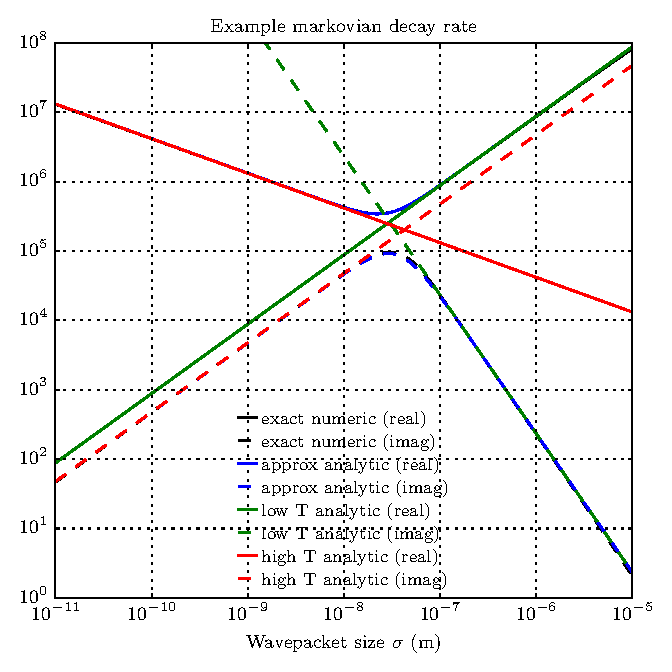
\includegraphics{figures/hidden_variables/decoherence_rate_example.pdf}
    \caption{Comparison of approximate analytic Markovian decoherence rate~\eqref{eq:gamma_total} and exact Markovian decoherence rate~\eqref{eq:markov_decoherence_factor_time_dep} between adjacent ($\upDelta m_F = \pm 1$) Zeeman sublevels of the $F=1$ ground state of a $^{87}$Rb atom in a $250\unit{G\,cm}^{-1}$ magnetic field gradient. Shown are the real (solid) and imaginary (dashed) parts of the small wavepacket limit (red) given by~\eqref{eq:gamma_pos_final} and large wavepacket limit (green) given by~\eqref{eq:gamma_vel_final}, their stitching together in the intermediate wavepacket regime (blue) given by~\eqref{eq:gamma_total} and the exact expression they approximate (black, not easily visible due to being similar to the blue curves) given by~\eqref{eq:markov_decoherence_factor_time_dep}. There is good agreement over all wavepacket sizes.}\label{fig:decoherence_rate_example}
\end{figure}

\subsection{Decoherence with mean auxiliary trajectories}\label{sec:spawned_trajectories}

A more accurate approach is to compute a decoherence factor at each timestep of the simulation by modelling the wavepackets as they accelerate away from each other, retaining in the model the position and velocity of each wavepacket. This inclusion of additional positions and velocities in the model comprises a minimal memory of the past interaction between the system and environment---that is, the internal and motional degrees of freedom of the atom.

In quantum mechanics there is not, in general, a single Gaussian wavepacket for each state, and even if the wavefunction corresponding to the originating state is a Gaussian wavepacket, transitions to other states at different times can produce an arbitrary superposition of Gaussian wavepackets in each other state. If we were to simulate this arbitrary superposition for all components of the multi-component wavefunction, we would not be saving any computational power at all, as we would have reverted to a fully quantum description of the motional degree of freedom, the antithesis of our intention. Therefore we draw the line at modelling a single trajectory for each state, in order to maintain simplicity whilst including at least some dynamics of the system--environment interaction.

Below I will talk about how to convert a decoherence factor at each point in time into a decoherence \emph{rate} at each point in time, that can be included in a differential equation for the state vector of the atom's internal state. Then I will introduce the averaging scheme I am using in order to turn what would be many trajectories for each state into one average trajectory.

Use of `auxiliary trajectories' for computing decoherence rates is common in the surface-hopping literature. There is a range of methods called `multiple spawning' methods, in which additional auxiliary trajectories regularly branch off the main trajectory (the one corresponding to the hidden variable), and are all considered in order to compute the overlap with the main wavepacket and hence the decoherence factor~\cite{doi:10.1021/jp994174i, doi:10.1063/1.476142, doi:10.1063/1.3103930}. These methods generally contain a parameter controlling the likelihood of new trajectories branching off, and trajectories can be discarded once they recede far enough from the main trajectory. If the parameter is tuned far enough, there can be so many auxiliary trajectories that an extremely accurate decoherence rate can be computed, though the computational cost in this case approaches that of a fully quantum simulation. A method by Shenvi \emph{et al.}~\cite{doi:10.1063/1.3575588}, like mine, tracks only one auxiliary trajectory per internal atomic state, probabilistically replacing them with newly spawned trajectories rather than simulating multiple auxiliary trajectories per state. However, the trajectories are spawned at specific moments---when the non-adiabatic coupling strength reaches a local maximum---leading to different behaviour in different locations in space. For example, if an atom were orbiting a magnetic field zero in a magnetic trap, this method would only spawn new trajectories at the orbit's point of closest approach, and decoherence rates would be inaccurate at other points in the orbit, even if the non-adiabatic coupling were still high throughout the orbit. My method has the potential to improve upon this due to the fact that it is in a sense spawning new trajectories all the time---rather than only at specific points in space as the method by Shenvi \emph{et al.}---and avoids the problem of an exponential proliferation of trajectories by only retaining a single, more-or-less representative trajectory for each state rather than many. 

\subsubsection{Decoherence rate in the absence of projective measurement}\label{sec:decoherence_without_projection}

Here we generalise our conception of the decoherence rate by removing the assumption that motional states are `reset' at each timestep. This resetting, which we assumed in Section~\ref{sec:continuous_projection}, set each motional state to be equal to $\ket{\phi_\eta(t)}$ at each timestep, and this led to all decoherence rates being zero due to the quantum Zeno effect (Section~\ref{sec:zeno_effect}). What is the reduction in the state amplitudes at each timestep if the wavepackets are not reset, but are left as arbitrary states? We know that if we were to perform a projective measurement at time $t$, the $i^\up{th}$ state amplitude would be reduced by a factor of $R_{\eta i}(t)$ compared to the original state amplitude $c_i(t)$ as in~\eqref{eq:R_projection}. If motional states are not reset at each timestep, then $R_{\eta i}(t)$ is not necessarily close to unity, as the wavepackets may be non-negligibly separated. In the absence of Hamiltonian evolution such that $\dv{c_i(t)}{t}=0$, the rate of change in $\tilde c_i(t)$ due to the changing decoherence factor is
\begin{align}
\dv{\tilde c_i(t)}{t} &= \dv{R_{\eta i}(t)}{t} c_i(t)\\
&= \frac1{R_{\eta i}(t)}\dv{R_{\eta i}(t)}{t} \tilde c_i(t).
\end{align}
and so we see that a decoherence rate that does not reset the environment states is the (negative of the) logarithmic derivative of the decoherence factor at any time, rather than just its derivative at $t=0$. This case encompasses the earlier case in which $R_{\eta i}(t) = 1$ at all times, in which case the logarithmic and ordinary derivatives are the same. Thus, given the decoherence factor between two states, along with its time derivative, we can compute a decoherence rate
\begin{align}
\gamma^\up{\textsc{mm}}_{ij}(t) =  -\frac1{R_{ij}(t)}\dv{R_{ij}(t)}{t},
\end{align}
such that in the absence of Hamiltonian evolution
\begin{align}
\dv{\tilde c_i(t)}{t} &= -\gamma^\up{\textsc{mm}}_{\eta i}(t)\,\tilde c_i(t),
\end{align}
where `\textsc{mm}'' stands for `minimal-memory'.

The (negative) logarithmic derivative of the decoherence factor~\eqref{eq:decoherence_factor} for the fixed-width Gaussian wavepackets gives the minimal-memory decoherence rates
\begin{align}
\gamma^\up{\textsc{mm}}_{ij}(t) = \left(
\frac{\vec r_{ij}}{4\sigma^2} + \frac\ii2\vec k_{ij}
\right)\cdot\dv{\vec r_{ij}(t)}{t}
+ \left(
\sigma^2\vec k_{ij} + \frac\ii2\vec r_{ij}
\right)\cdot\dv{\vec k_{ij}(t)}{t},
\end{align}
which for a given relative acceleration $\vec a_{ij}$ between the states, and written in terms of relative velocity instead of wavenumber, is
\begin{align}\label{eq:mm_decoherence_rate}
\gamma^\up{\textsc{mm}}_{ij}(t) = 
\frac{1}{4\sigma^2}\vec r_{ij}(t)\cdot\vec v_{ij}(t)
+ \frac{\sigma^2 m^2}{\hbar^2}\vec v_{ij}(t)\cdot\vec a_{ij}(t)
+ \ii\frac{m} {2\hbar} \left(\abs{\vec v_{ij}(t)}^2 + \vec r_{ij}(t)\cdot \vec a_{ij}(t)\right),
\end{align}\label{eq:minimal_memory_decoherence_rate}
where $\vec r_{ij}(t) = \vec r_i(t) - \vec r_j(t)$ and $\vec v_{ij}(t) = \vec v_i(t) - \vec v_j(t)$ are the relative position and velocity of the two states, and $\vec a_{ij}(t)$ is their relative acceleration:
\begin{align}
\vec a_{ij}(t) = -\frac1 m\left(\nabla V_i(\vec r_i, t) - \nabla V_j(\vec r_j, t)\right).
\end{align}
Note this is slightly different to the relative acceleration used in the Markovian decoherence calculation in Section~\ref{sec:markovian_decoherence}. Here, we actually have (approximate) positions $\vec r_i(t)$ and $\vec r_j(t)$ for both states' wavepackets, and so we can evaluate the potential gradient separately at the two positions rather than having to use the position of the state currently selected by the hidden variable for both.

Equation~\eqref{eq:minimal_memory_decoherence_rate} is our minimal-memory decoherence rate, and requires as input the centre-of-mass position and velocity of each Gaussian wavepacket as input. Let's now move on to how these trajectories are computed.

\subsubsection{From many trajectories, one}

As mentioned, this method track only one trajectory per state. However, it continuously considers the spawning of new trajectories, and rather than actually tracking multiple trajectories per state or probabilistically replacing the existing trajectories with the new ones, it simply averages the trajectories together, weighted by their quantum probabilities. At the end of each timestep, positions and velocities (other than those of the main trajectory) are updated according to a weighted sum of their present values and those of the main trajectory:
\begin{align}\label{eq:position_averaging}
\vec r_{i\neq\eta}(t^\prime) &\leftarrow 
  Q_{i\eta}(t^\prime, t)\,\vec r_\eta(t^\prime)
  + \left(1 - Q_{i\eta}(t^\prime, t)\right)\vec r_i(t^\prime),\\
\vec v_{i\neq\eta}(t^\prime) &\leftarrow
  Q^\up{time}_{i\eta}(t^\prime, t)\vec v_\eta(t^\prime)
  + \tilde Q^\up{space}_{i\eta}(t^\prime, t)(\vec v_\eta(t^\prime) + \upDelta \vec v_{i\eta}(t^\prime))\nonumber\\
  &\phantom{\rightarrow} + \left(1 - Q^\up{time}_{i\eta}(t^\prime, t) - \tilde Q^\up{space}_{i\eta}(t^\prime, t)\right)\vec v_i(t^\prime),
  \label{eq:velocity_averaging}
\end{align}
where $Q_{i\eta}(t^\prime, t) = P_{i\eta}(t^\prime, t)/\abs{c_i(t^\prime)}^2$ is the fraction of the population\footnote{Note that $\abs{c_i(t^\prime)}^2$ is the $i^\up{th}$ population at time $t^\prime$ due to unitary evolution only over the time interval, without taking into account decoherence, since all population flows are computed from unitary evolution only and decoherence is treated separately.} of state $i$ at time $t^\prime$ that flowed to it from state $\eta$ in the interval $t$ to $t^\prime$, with $Q_{i\eta}^\up{time}(t^\prime, t)$ and $\tilde Q_{i\eta}^\up{space}(t^\prime, t)$ defined similarly in terms of $P_{i\eta}^\up{time}$ and $\tilde P_{i\eta}^\up{time}$ as defined in Section~\ref{sec:velocity_correction}, and where $\upDelta \vec v_{i\eta}(t^\prime)$ is the required velocity correction for a transition from state $\eta$ to state $i$ at time $t^\prime$, as discussed in Section~\ref{sec:velocity_correction}:
\begin{align}\label{eq:non_markovian_velocity_jump}
\upDelta \vec v_{i\eta}(\vec r, t^\prime) = \left[\sgn(\vec v\cdot \hat{\vec d}_{i\eta})
\sqrt{(\vec v\cdot \hat{\vec d}_{i\eta})^2 + \frac2m\left(V_i(\vec r, t^\prime) - V_\eta(\vec r, t^\prime)\right)} - (\vec v\cdot \hat{\vec d}_{i\eta}),
\right]\hat{\vec d}_{i\eta},
\end{align}
where $\vec r = \vec r_\eta(t^\prime)$ and $\vec v = \vec v_\eta(t^\prime)$ are the position and velocity of the main trajectory at time $t^\prime$, and the non-adiabatic coupling unit vector $\hat{\vec d}_{i\eta} = \hat{\vec d}_{i\eta}(\vec r_\eta(t^\prime))$ is evaluated at the position along the main trajectory at time $t^\prime$.

The above scheme is constructed to track a mean trajectory for each state, where `mean' is defined as a weighted sum of positions and velocities with those of the main trajectory whenever transitions from the latter occur, taking into account velocity jumps and frustrated transitions, with the energy conservation calculation for the velocity jumps based on the potentials at the location of the main trajectory.

\subsection{What are we `following' exactly?}\label{sec:dirac_deltas}

Now that we've worked out a way to approximate the result of projecting the multi-component wavefunction onto a specific motional state (a Gaussian wavepacket) without resetting all motional states (also Gaussian wavepackets) to be equal to the one we are projecting onto, why not take the process further? We can use the same method to project onto any wavefunction we like, in order to inspect what the multi-component wavefunction looks like projected onto the wavefunction in question. This does not have to imply anything about the form of the motional states, which remain Gaussians at all times. It just defines what we `see' at each timestep of our simulation.

For example, if we projected onto a Dirac delta, that would tell us what the multi-component wavefunction looks like at a specific point in space, say, the centre-of-mass position of the wavepacket corresponding to the hidden variable.

This is appealing for several reasons. Firstly, consider the projected Hamiltonian $\hat H_\eta(t)$ first introduced in Section~\ref{sec:continuous_projection}. Since we do not want to have to actually construct Gaussian wavepackets in order to compute the integral that defines the projected Hamiltonian, our only recourse is to approximate the projected Hamiltonian as the value of the full Hamiltonian at the centre-of-mass position of the main trajectory's Gaussian wavepacket:
\begin{align}
\matrixel{\chi_i}{\hat H_{\eta}(t)}{\chi_j} &= \matrixel{\chi_i\ \phi_\eta(t)}{\hat H(t)}{\chi_j\ \phi_\eta(t)}\\
&\approx \matrixel{\chi_i\ \vec r_\eta(t)}{\hat H(t)}{\chi_j\ \vec r_\eta(t)}\\
&\equiv H_{ij}(\vec r_\eta, t),
\end{align}
which can be considered a small-wavepacket approximation, as mentioned in Section~\ref{sec:semiclassical_methods} in the context of the Ehrenfest semiclassical model. If an arbitrary position is used in place of $\vec r_\eta$, this results in an operator valued function of space $\hat H(\vec r, t)$, which operates only on the internal degrees of freedom of the atom.

This is the operator we actually use in the algorithm, and with it, there are no longer any Gaussian wavepackets to compute integrals over or anything else---all details of the wavepackets are encapsulated and parametrised by the approximations and analytics in this and the preceding sections, leaving us to focus on the classical dynamics of the atoms' centre-of-mass motion and the quantum evolution of their internal states according to $\hat H(\vec r, t)$ evaluated at the classical positions (representing the centre-of-mass position of the wavepackets) of the atoms.

Although this can be considered a small wavepacket approximation, we cannot use arbitrarily small wavepacket sizes in our decoherence calculations, as the decoherence rates (under both the Markovian and auxiliary trajectories approaches) do not converge to a constant as the wavepacket sizes decrease---rather they become arbitrarily large. Very high spin decoherence rates have the potential to prevent spin flips altogether, also a result of the quantum Zeno effect, since high decoherence rates imply strong measurement, and strong measurement of an observable prevents evolution of that variable.\footnote{I have sometimes wondered if there is a way to harness this to prevent Majorana losses in evaporation to \textsc{bec}, by measuring very strongly whether they have occurred.} So there is a possible inconsistency here: can we make the wavepackets small or not?

On the other hand, note in~\figref{fig:decoherence_rate_example} the trend in the Markovian decoherence rate as wavepackets become large: the decoherence rate becomes large as well. The expression for the minimal-memory non-Markovian decoherence rate~\eqref{eq:mm_decoherence_rate} also yields a large decoherence rate for large wavepackets. In both cases this is decoherence due to separation in velocity space. While this is the correct result given our assumptions, it causes problems when combined with the above method of approximating the projected Hamiltonian. Essentially, rapid velocity-induced decoherence occurs when the wavepackets are large because spatially large Gaussians are small in velocity space, and hence do not need to accelerate much to be no longer overlapping in velocity space. But do we really expect our wavepackets to be minimal uncertainty wavepackets? Certainly not when they are large compared to the structure of a spatially-varying Hamiltonian. A real wavepacket, whilst undergoing a transition to another state, does not do so everywhere in space the same, as in a single-mode approximation, but our formulation so far assumes it does. In the limit of a very large spin-$\frac12$ wavepacket undergoing a complete Majorana spin flip due to a magnetic field zero for example, would appear, as its centre-of-mass passed over the zero, as approximately two half-Gaussians, one in each state. It is doubtful that such spatially complex wavepackets have narrow enough velocity distributions to lead to decoherence rates as high as the expressions we've derived so far suggest. Narrow velocity distributions are therefore inconsistent with the other assumptions of our model and any consequences of rapid velocity separation in the model should be viewed with scepticism.

Another argument is that, if two wavepackets are co-located in space but not in velocity space, the amplitude of one of them as seen from the centre-of-mass position of the other is not zero. It's the fact that their relative phase varies so much over the extent of the wavepackets that causes their projection onto each other to be small when their velocities are very different.\footnote{Some call this `dephasing' to distinguish from other forms of decoherence.} So it's only after this averaging process---integrating over all space---that the wavepackets look like they are small from each other's perspective. One of the common themes of this method as a whole is that we are often happy with \emph{representative} results rather than average ones, drawing results from approximately correct statistical distributions, and only observing the complete distribution when we analyse a large sample of results. Continuing in this vein, why not consider the value of the multi-component wavefunction along a specific trajectory in space, rather than its projection onto a Gaussian? The projection of a multi-component wavefunction onto a Gaussian isn't any more useful or intuitive a quantity than tracing a curve through spacetime and asking ``what is the wavefunction here?" This way, instead of a simulation telling us ``There was, on average, no population transfer to such-and-such state", it would give a (more likely to be useful in my opinion) answer ``there was a lot of population transfer to this state, but the phase is essentially random". 

The final argument is empirical: attempts to implement the model with the Gaussian projections do not work well unless wavepackets are small. The decoherence rates are too high, presumably for the speculative reasons discussed above. This damps the population of states other than that selected by the hidden variable too quickly, such that the simulated population of a state is zero even though according to the Schr\"odinger wave equation it should not be (it merely has an inhomogeneous phase). Simply deleting the terms caused by velocity separation from the decoherence rate expressions improves the results somewhat. But if projecting onto a Dirac delta instead, there are no velocity-separation terms to argue for the deletion of, and one obtain modestly better results in any case (as shown in Section~\ref{sec:HVSC_results}).

Shenvi \emph{et al.}~\cite{doi:10.1063/1.3575588} also seem to find the velocity-separation term of their decoherence factor troublesome, and opt to remove it by gauge transforming the wavepackets to have the same velocity. They argue that because at least a small initial velocity difference between wavepackets is required by energy conservation (i.e.~the velocity jumps from Section~\ref{sec:velocity_correction}), that it is `unfair' to have an initial sudden drop in coherence because of this. I agree that an immediate drop in coherence upon a transition is strange, but this is small compared to the decoherence that large Gaussian wavepackets undergo upon further acceleration away from each other, which also seems unphysically large and needs to be addressed as well. But velocity jumps or not, these are the actual decoherence factors between pairs of Gaussians, and if we don't like the answer, perhaps the projection of the total wavefunction onto a Gaussian isn't the question we meant to ask. Perhaps we should be asking simply what value a multi-component wavefunction has at a specific point in space. Shenvi \emph{et al.}~gauge transform away the entire velocity difference between the wavepackets, not only the part of it mandated by energy conservation, leading me to suspect that some of the same concerns I outlined above occurred to them too, or that they simply observed, like me, that the velocity separation was responsible for what appeared to be unphysically large decoherence rates in their results.

In light of all this, I now redefine `follow' to mean ``look at the wavefunction's value at the centre-of-mass position of the classical trajectory corresponding to the state being followed", the result of which can be computed by projecting the total wavefunction onto a Dirac delta, resulting in a decoherence factor
\begin{align}
R^{\textsc{dd}}_{ij}(t) = \braket{\vec r_i(t)}{\phi_j(t)}
\end{align}
where $\ket{\phi_j(t)}$ is one of our usual Gaussian motional states and \textsc{dd} stands for `Dirac delta'. Following identical arguments to the previous two sections, we obtain Dirac-delta decoherence rates for the Markovian case as
\begin{align}\label{eq:markovian_decoherence_rate_dd}
\gamma^\up{Markov\,\textsc{dd}}_{ij}(\vec r, t) \approx \frac1{2\upGamma(\frac54)}\sqrt{\frac{\abs{\vec a_{ij}(\vec r, t)}}{\sigma}} + \ii\frac1{2\upGamma(\frac54)^2}\frac{m\sigma\abs{\vec a_{ij}(\vec r, t)}}{\hbar},
\end{align}
which is identical to the position-only approximation~\eqref{eq:gamma_pos_final} up to a factor of $2^{\frac14}$, and for minimal-memory non-Markovian case as 
\begin{align}\label{eq:minimal_memory_decoherence_rate_dd}
\gamma^\up{\textsc{mmdd}}_{ij}(t) = \frac1{2\sigma^2}\vec r_{ij}(t)\cdot\vec v_{ij}(t)
                        - \ii \frac m\hbar\vec r_{ij}(t)\cdot \vec a_{ij}(t),
\end{align}
with all symbols as defined in Section~\ref{sec:markovian_decoherence} and Section~\ref{sec:spawned_trajectories}, respectively.

Now that we are projecting onto a Dirac delta instead of a Gaussian, calculation of the projected Hamiltonian as simply the value of the full Hamiltonian at a specific point in space is no longer a contradiction, as it is exactly what we would get if we projected the full Hamiltonian onto a Dirac delta instead of a Gaussian.


\section{Algorithms}\label{sec:HVSC_algorithm}

Now we have presented all the pieces from which the two versions of the hidden-variable semiclassical method are constructed. In this section I present step-by-step instructions for implementing the two versions of the method---one using Dirac-delta Markovian decoherence, and the other using auxiliary trajectories with Dirac-delta minimal-memory decoherence.

\subsection{Markovian hidden-variable semiclassical method}\label{sec:algo_markovian}
This is the simplest version of my method, using crude Markovian decoherence as discussed in Section~\ref{sec:markovian_decoherence}, and simulating only one trajectory corresponding to the centre-of-mass motion of the state corresponding to the hidden variable at each moment in time.

\subsubsection{State variables}
The Markovian variant of the hidden-variable semiclassical method has the following state variables describing the state of each simulated atom at each moment of time:
\begin{itemize}
    \item The internal state vector of the atom $\ket{\tilde\chi(t)}$, in any chosen basis (though the local eigenbasis is likely to be computationally simplest to perform calculations in).
    \item The position $\vec r(t)$ and velocity $\vec v(t)$ of the atom.
    \item The hidden variable $\eta(t)$, equal to an integer index specifying one of the eigenstates $\ket{\chi_\eta(\vec r, t)}$ of the Hamiltonian $\hat H(\vec r, t)$ atom in the local energy eigenbasis.
\end{itemize}

\subsubsection{Initial conditions}

Strictly, the hidden-variable semiclassical method is intended to simulate the classical centre-of-mass motion of thermal wavelength sized Gaussian wavepackets. Therefore the initial conditions for the positions and velocities of the atoms in an ensemble are arbitrary, classical initial conditions, and so one might draw them, along with the internal states, randomly from a Boltzmann distribution for a given confining potential and temperature, such that the initial internal state of each atom is an eigenstate $\ket{\chi_i(\vec r, t=0)}$. In this case the initial value $\eta(t=0)$ of the hidden variable for each atom should correspond to its chosen eigenstate.

However, one might want to convert an initial \emph{wavefunction} into an ensemble of positions and velocities, in which case one can draw positions and momenta from the quantum probability distributions $\matrixel{\psi(t=0)}{\hat{\vec r}}{\psi(t=0)}$ and $\matrixel{\psi(t=0)}{\hat{\vec p}}{\psi(t=0)}$ for an initial motional state vector $\ket{\psi}$.
Similarly, one can set the initial internal state vector of each atom to an arbitrary desired internal state vector appropriate for the problem at hand, in which case the initial values of the hidden variable for each atom in an ensemble being simulated should be chosen randomly with probability equal to the internal state populations $\abs{\braket{\chi_i(\vec r, t=0)}{\tilde\chi(\vec r, t=0)}}^2$ in the local basis at the position of each atom.
More complex initial conditions are possible; there is no reason why one can't draw positions, velocities and internal states from arbitrary joint probability distributions, or use hand-crafted initial states, provided that the hidden variables are chosen randomly at the end with probabilities equal to the internal state populations in the local basis of each atom so as to be consistent with the Born rule.

\subsubsection{Evolution}

Evolving the Markovian hidden-variable semiclassical method involves three coupled differential equations, a stochastic evolution rule, and some additional steps to be performed in between numerical integration steps. Because the modifications in between steps can be discontinuous, multi-step integration schemes that retain information from previous integration steps should be avoided. One step of the Markovian hidden-variable semiclassical method comprises the following steps to evolve the state variables from time $t$ to $t^\prime = t + \upDelta t$, where $\upDelta t$ is small compared to dynamical timescales of the problem.

\begin{enumerate}
    \item Evolve the internal state vector and motional state variables of each atom from time $t$ to $t^\prime$ according to the following coupled differential equations, using one or more steps of your favourite non-multi-step numerical integration method:
    \begin{align}
    \dv{t}\ket{\tilde\chi(t)} &= -\frac\ii\hbar \hat H(\vec r, t)\ket{\tilde\chi(t)} - \hat\Gamma^\up{Markov\,\textsc{dd}}_\eta(\vec r, t)\ket{\tilde\chi(t)},\\
    \dv{t}\vec v(t) &= -\frac1m\nabla V_\eta(\vec r, t),\\
    \dv{t}\vec r(t) &= \vec v(t),
    \end{align}
    where $V_\eta(\vec r, t)$ is the (space- and/or time-dependent) eigenvalue of $\hat H(\vec r, t)$ corresponding to the eigenstate $\ket{\chi_\eta(\vec r, t)}$, and the Markovian decoherence operator is
    \begin{align}
    \hat\Gamma^\up{Markov\,\textsc{dd}}_\eta(\vec r, t) = \sum_i\ketbra{\chi_i(\vec r, t)}{\chi_i(\vec r, t)}\gamma^\up{Markov\,\textsc{dd}}_{\eta i}(\vec r, t),
    \end{align}
    where $\gamma^\up{Markov\,\textsc{dd}}_{ij}(\vec r, t)$ are the approximate Markovian decoherence rates given by~\eqref{eq:markovian_decoherence_rate_dd}. The integration of the internal state can be performed in the local eigenbasis using the transformed Hamiltonian defined in~\eqref{eq:Tully_adiabatic_schro}, in which case the decoherence operator is diagonal with the $i^\up{th}$ diagonal equal to $\gamma^\up{Markov\,\textsc{dd}}_{\eta i}(\vec r, t)$.

    \item Normalise the internal state vector to unit norm:
    \begin{align}
    \ket{\tilde\chi(t^\prime)} \leftarrow \frac{\ket{\tilde\chi(t^\prime)}}
                               {\sqrt{\braket{\tilde\chi(t^\prime)}{\tilde\chi(t^\prime)}}}
    \end{align}

    \item Evaluate the $S^\up{time}$, $S^\up{space}$ and $S^\up{stay}$ matrices over this time interval for Tully's minimal-switches algorithm as described in Section~\ref{sec:fewest_switches}, equations~(\ref{eq:S_space}--\ref{eq:S_stay}). This may require numerical differentiation of the basis vectors of the Hamiltonian with respect to space and time, and possibly numerical diagonalisation of the Hamiltonian to obtain the basis vectors as functions of space and time, if analytic expressions are not known. If $\upDelta t$ is not small enough to be considered infinitesimal for the purposes of evaluating~\eqref{eq:q_space} and~\eqref{eq:q_time}, and one numerically integrates them for a more accurate result, note that these expressions require the state populations $\{c_i(t)\}$ in the local basis in the \emph{absence} of decoherence; one therefore cannot do this integral in tandem with integrating the above differential equation for the internal state.\footnote{Though with split-operator methods and some care, the decoherence term can be treated separately such that the two integrals can be evaluated without repeating calculations unnecessarily.} Alternately, compute the overall $S$ matrix of your favourite hidden-variable theory for evolution over the given time interval in the local eigenbasis (similarly keeping in mind that the effective unitary given to the hidden-variable theory must be due to the evolution of $\hat H_\up{eff}(t)$ only, and not the decoherence term). If it saves computational power to do so, only compute column $\eta$ of $S$, since only transitions from state $\eta$ to other states need be considered.

    \item Compute $\tilde P^\up{space}$~\eqref{eq:tilde_P_space} and hence $\tilde S^\up{space}$~\eqref{eq:tilde_S_space} to set the probability of classically disallowed transitions to zero as described in Section~\ref{sec:velocity_correction}.

    \item Modify the hidden variable with probability
    \begin{align}
    \Pr(\eta\toverset{\up{space}}\rightarrow i) &= \tilde S^\up{space}_{i\eta}
    \end{align}
    that it transitions to the state ($i\neq\eta$) via a spatially induced transition, and probability
    \begin{align}
    \Pr(\eta\toverset{\up{time}}\rightarrow i) &= S^\up{time}_{i\eta}
    \end{align}
    that it transitions to a state ($i\neq\eta$) via a temporally induced probability, and probability
    \begin{align}
    \Pr(\eta\rightarrow\eta) &= 1 - \sum_i \left(\tilde S^\up{space}_{i\eta} + S^\up{time}_{i\eta}\right)
    \end{align}
    that it keeps its current value. These choices can be randomly chosen between with the correct probabilities as described in~\figref{fig:random_choice}.

    \item If the hidden variable did transition to a different state $i\neq\eta$, and if it was a spatially induced transition, instantaneously adjust the atom's velocity as required by energy conservation:
    \begin{align}
    \vec v(t^\prime) \leftarrow \vec v(t^\prime) + \upDelta \vec v_{\eta i}(\vec r, t),
    \end{align}
    where $\upDelta \vec v_{\eta i}(\vec r, t)$ is given by~\eqref{eq:velocity_jump}.
\end{enumerate}

This completes the Markovian hidden-variable semiclassical method.

\subsection{Mean auxiliary trajectories hidden-variable semiclassical method}\label{sec:algo_non_markovian}

This is the more complex version of my method. Additional classical trajectories are propagated---one for each internal state of each atom---but other than classically evolving these additional trajectories, the increase in computational cost is minimal.

\subsubsection{State variables}
The non-Markovian/Mean auxiliary trajectories variant of the hidden-variable semiclassical method has the following state variables describing the state of each simulated atom at each moment of time:
\begin{itemize}
    \item The internal state vector of the atom $\ket{\tilde\chi(t)}$, in any chosen basis (though the local eigenbasis is likely to be computationally simplest to perform calculations in).
    \item A set of positions $\{\vec r_i(t)\}$ and velocities $\{\vec v_i(t)\}$, one position and velocity for each internal state of the atom.
    \item The hidden variable $\eta(t)$, equal to an integer index specifying one of the eigenstates $\ket{\chi_\eta(\vec r_\eta, t)}$ of the Hamiltonian $\hat H(\vec r_\eta, t)$ atom in the local energy eigenbasis at the location $\vec r_\eta$ of the main trajectory.
\end{itemize}

\subsubsection{Initial conditions}
The manner of generating initial conditions of the mean auxiliary trajectories variant of the hidden-variable semiclassical method is identical to that of the Markovian variant, with the exception that multiple initial positions and velocities are required instead of just one. The initial positions and velocities of all auxiliary trajectories can however simply be set equal to those of the main trajectory for each atom.

\subsubsection{Evolution}

The evolution of the state variables for each atom from time $t$ to $t^\prime = t + \upDelta t$ in the non-Markovian hidden-variable semiclassical method proceeds similarly to the Markovian variant.

\begin{enumerate}
    \item Evolve the internal state vector and set of motional state variables of each atom from time $t$ to $t^\prime$ according to the following coupled differential equations, using one or more steps of your favourite non-multi-step numerical integration method:
    \begin{align}
    \dv{t}\ket{\tilde\chi(t)} &= -\frac\ii\hbar \hat H(\vec r_\eta, t)\ket{\tilde\chi(t)} - \hat\Gamma^\up{\textsc{mmdd}}_\eta(t)\ket{\tilde\chi(t)},\\
    \dv{t}\vec v_i(t) &= -\frac1m\nabla V_i(\vec r_i, t),\\
    \dv{t}\vec r_i(t) &= \vec v_i(t),
    \end{align}
    where $V_i(\vec r_i, t)$ is the (space- and/or time-dependent) eigenvalue of $\hat H(\vec r_i, t)$ corresponding to the eigenstate $\ket{\chi_i(\vec r_i, t)}$ at the position of the $i^\up{th}$ trajectory, which may be the main ($i=\eta$) or an auxiliary ($i\neq\eta$) trajectory; and the non-Markovian decoherence operator is
    \begin{align}
    \hat\Gamma^\up{\textsc{mmdd}}_\eta(t) = \sum_i\ketbra{\chi_i(\vec r_\eta, t)}{\chi_i(\vec r_\eta, t)}\gamma^\up{\textsc{mmdd}}_{\eta i}(t),
    \end{align}
    where $\gamma^\up{\textsc{mmdd}}_{ij}(t)$ are the minimal-memory non-Markovian decoherence rates given by~\eqref{eq:minimal_memory_decoherence_rate_dd}; $\gamma^\up{\textsc{mmdd}}_{\eta j}(t)$ comprising the diagonals of $\hat\Gamma^\up{\textsc{mmdd}}_\eta(t)$ if working in the local eigenbasis along the main trajectory. When computing $\gamma^\up{\textsc{mmdd}}_\eta(t)$, clip its real part from below to zero. Although such recoherence can in principle be physically meaningful, it can arise out of tiny amplitudes of states with auxiliary trajectories far from the main trajectory, and is hence subject to large floating-point error.\footnote{Large error in \emph{positive} (real parts of) decoherence rates in the same context is not a problem, as the state amplitudes are already very close to zero, so the accuracy of the rate at which they more closely approach zero is of no consequence.} I have not observed this problem with the Dirac delta based decoherence rates, but it does seem to appear if the Gaussian-projection based decoherence rates are used.

    \item Normalise the internal state vector to unit norm:
    \begin{align}
    \ket{\tilde\chi(t^\prime)} \leftarrow \frac{\ket{\tilde\chi(t^\prime)}}
                               {\sqrt{\braket{\tilde\chi(t^\prime)}{\tilde\chi(t^\prime)}}}
    \end{align}

    \item Evaluate the $S^\up{time}$, $S^\up{space}$ and $S^\up{stay}$ matrices as in Step 3 for the Markovian case 

    \item Compute $\tilde S^\up{space}$ as in Step 4 for the Markovian case. We treat transitions to have occurred at the location of the originating trajectory, therefore for the purposes of computing $\tilde S^\up{space}$, the expressions for $\upDelta v^2_{ij}(\vec r, t)$~\eqref{eq:delta_v_squared} and $\hat{\vec d}_{ij}(\vec r, t)$~\eqref{eq:non_adiabatic_coupling_vector} must be evaluated using $\vec r = \vec r_i(t^\prime)$, and the conditional in $\tilde P^\up{space}$~\eqref{eq:tilde_P_space} evaluated with $\vec v = \vec v_i(t^\prime)$. Since only transitions from the current state specified by the hidden variable to other states need to be considered, one only needs to compute column $\eta$ of $\tilde S^\up{space}$, in which case only $\vec r_\eta$ and $\vec v_\eta$ are necessary. This is then identical to the non-Markovian case, in which the main trajectory is the only trajectory simulated.

    \item Compute the energy-conservation mandated velocity difference $\upDelta\vec v_{\eta i}$ given by~\eqref{eq:velocity_jump} for all $i\neq\eta$. As with Step 4, since we treat transitions to have occurred at the location of the main trajectory, the velocity difference expression should be evaluated using the position and velocity of the main trajectory, as emphasised in~\eqref{eq:non_markovian_velocity_jump}. 

    \item Instantaneously modify the positions and velocities of all auxiliary trajectories ($i\neq\eta$) according to~\eqref{eq:position_averaging} and~\eqref{eq:velocity_averaging}. This in essence spawns new auxiliary trajectories at the location of the main trajectory, but does not keep them: the averaging expressions replace each auxiliary trajectory with a weighted sum of its previous position and velocity and the position and velocity of the new trajectory. If the population of the state corresponding to a given auxiliary trajectory falls below some threshold (I use $\abs{c_{i\neq\eta}(t)}^2 < 10^{-8}$), then discard the trajectory and replace it with the position and velocity of the main trajectory.

    \item Probabilistically make a transition of the hidden variable as in Step 5 for the Markovian case.
    
    \item In the case that the hidden variable transitioned, replace the trajectory of the new state with the position and velocity of the previous main trajectory.
    In the case that it was a spatially-induced non-adiabatic transition, adjust the velocity of the new state's trajectory with the previously computed $\upDelta\vec v_{\eta\xi}$, where $\eta$ is the previous value of the hidden variable and $\xi$ is the new value.
   
\end{enumerate}

This completes the mean auxiliary trajectories hidden-variable semiclassical method.

\section{Results}\label{sec:HVSC_results}

Here I demonstrate the two variants of the method, each for two different spatially dependent Hamiltonians in one dimension, and compare them to the numerical result from the full Schr\"odinger wave equation. All simulations are for $^{87}$Rb atoms in the $F=1$ ground state subject to the Zeeman Hamiltonian for a given magnetic field profile. In scenario I, atoms in the trapped state (for $^{87}$Rb, the locally spin-down sate is magnetically trappable) pass over a field minimum, which induces Majorana transitions, allowing the spin-flipped atoms to escape. In scenario II, the magnetic field profile is modified to create two closely spaced field minima. This scenario demonstrates the importance of accurate decoherence in surface-hopping/hidden-variable semiclassical methods, as the two regions of non-adiabatic coupling are encountered in a time comparable to the decoherence timescale where the exact form of the decoherence model can strongly influence the outcome of transitions. I use Schr\"odinger theory for the hidden-variable theory throughout. Since the Hamiltonians are time-independent, as mentioned these results do not test my proposed method of conditionally applying velocity jumps to transitioned atoms---velocity jumps are always applied.

I simulated both scenarios first using the Schr\"odinger wave equation, as the gold-standard against which to benchmark the other methods. Numerically I solved for the three-component wavefunction using fourth-order Runge--Kutta (Section~\ref{sec:rk4}) and the Fourier method of evaluating spatial derivatives (Section~\ref{sec:fourier_pseudospectral}). I added imaginary potentials near the boundaries of the region I wished to simulate to absorb untrapped wavepackets rather than have them reflect or wrap around due to periodic boundary conditions inherent in the Fourier method of derivatives. The initial condition was a Gaussian wavepacket in the locally spin-down eigenstate, $m_F = -1$, though I simulated in the fixed eigenbasis of $\hat F_z$, transforming as necessary to create the initial conditions, and later to compare state populations in the local eigenbasis.

I then simulated both scenarios with $10^4$ semiclassical atoms using the Ehrenfest semiclassical method (Section~\ref{sec:sterngerlachseparation}), the Markovian hidden-variable semiclassical method (Section~\ref{sec:algo_markovian}), and the mean auxiliary trajectories hidden-variable semiclassical method (Section~\ref{sec:algo_non_markovian}). The initial conditions were set by drawing positions and velocities randomly for each semiclassical particle from the position and velocity probability distributions implied by the Gaussian wavepacket.

For both semiclassical methods I used simple first-order split-step evolution (Section~\ref{sec:split-step}) for the quantum evolution in the local eigenbasis, and evolved the classical trajectories analytically using constant acceleration over each timestep:
\begin{align}
\ket{\tilde\chi_H(t^\prime)} &\approx \ee^{-\hat\Gamma_\eta(t)\upDelta t}\hat U_H(z^\prime, t^\prime)\,\hat U_H^\dagger(z, t)\,\ee^{-\frac\ii\hbar \hat V(z, t)\upDelta t}\ket{\tilde\chi_H(t)},\\
z^\prime &\approx z - \frac{\upDelta t^2}{2m}\nabla V_\eta(z)\\
v^\prime &\approx v - \frac{\upDelta t}{m}\nabla V_\eta(z),
\end{align}
where $z$, $v$ and $t$ are the position, velocity and time at the start of a timestep, $z^\prime$, $v^\prime$ and $t^\prime$ at the end of the timestep, and $\upDelta t = t^\prime - t$, is the timestep, which was $\upDelta t = 500\unit{ns}$. These methods are not particularly accurate, but were sufficient for these demonstrations and allowed the implementation to be simple. In particular, the ordering of the individual operators for evolving the state vector over a timestep was chosen to allow everything to the right of the decoherence factor be the unitary part of the evolution for the timestep, which could be input to Schr\"odinger theory as the unitary describing evolution in the local basis for that timestep.

A summary of all the simulation results presented in this section is given in Table~\ref{table:figure_summary}.

\subsubsection{Scenario I}

In this scenario, a $^{87}$Rb atom begins as an initially stationary Gaussian wavepacket of width $600\unit{nm}$ (equal to the thermal de~Broglie wavelength at $T=0.2\unit{\upmu K}$) centred at $z_0 = -20\unit{\upmu m}$ in the Zeeman potential experienced by the $F=1$ ground-state manifold (Section~\ref{sec:zeeman_sublevels}) with the following magnetic field profile:
\begin{align}
\vec B_\up{trap}(z) = (B_x, B_y, B_z) = \left(B_\perp, 0, B_z^\prime z\right)
\end{align}
where the transverse magnetic field is $B_\perp = 162.5\unit{mG}$ and the $z$-gradient is $B_z^\prime = 250\unit{G\,cm^{-1}}$. This potential provides a region close to $z=0$ where the magnetic field rapidly reverses direction too quickly for the atom's spin to adiabatically follow, inducing Majorana transitions. The atom accelerates under the initial potential gradient toward this region. The adiabatic potentials resulting from the Zeeman Hamiltonian with this magnetic field are shown in~\figref{fig:scenario_1}. Results are shown in Figure~\ref{fig:scenario_one_markovian} for the Markovian model and Figure~\ref{fig:scenario_one_aux} for the auxiliary trajectories model.

\begin{figure}[h]
    \centerfloat
    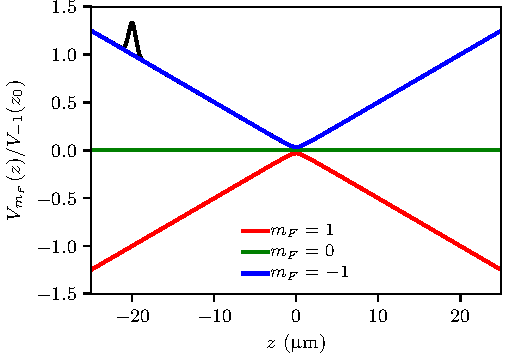
\includegraphics{figures/hidden_variables/scenario_1.pdf}
    \caption{Adiabatic potentials for scenario I with a single region of coupling. The initial probability distribution of the atoms is depicted (in arbitrary units), offset for clarity by the adiabatic potential of the initial state.}\label{fig:scenario_1}
\end{figure}
\begin{figure}[h]
    \centerfloat
    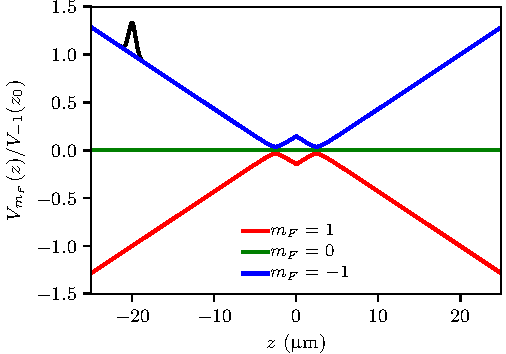
\includegraphics{figures/hidden_variables/scenario_2.pdf}
    \caption{Adiabatic potentials for scenario II, with two closely spaced coupling regions. The initial probability distribution of the atoms is depicted (in arbitrary units), offset for clarity by the adiabatic potential of the initial state.}\label{fig:scenario_2}
\end{figure}
\subsubsection{Scenario II}
Scenario II is identical to scenario I, except that the magnetic field profile is instead\footnote{This magnetic field profile is unphysical---though similar Hamiltonians can be constructed by means of dressed potentials using fast-rotating fields---it serves as a good test that highlights the improvement of the mean auxiliary trajectories method over the Markovian method.}
\begin{align}
\vec B_\up{trap}(z) = (B_x, B_y, B_z) = \begin{cases}
\left(B_\perp, 0, B_z^\prime (z + z_\up{fieldmin})\right) & z < 0\\
\\
\left(B_\perp, 0, -B_z^\prime  (z + z_\up{fieldmin})\right) & z >= 0
\end{cases}
\end{align}
where $z_\up{fieldmin} = 2.5\unit{\upmu m}$ is the distance of each field minimum to the origin, such that the two minima are separated by $5\unit{\upmu m}$, and with the other variables having the same values as in scenario I. The adiabatic potentials resulting from the Zeeman Hamiltonian with this magnetic field are shown in~\figref{fig:scenario_2}. Results are shown in Figure~\ref{fig:scenario_two_markovian} for the Markovian model and Figure\ref{fig:scenario_two_aux} for the auxiliary trajectories model.

\afterpage{
\newgeometry{left=1in,bottom=1.5in,right=1in,top=1.5in}
\begin{landscape}% Landscape page
\begin{table}
    \renewcommand{\arraystretch}{1.5}
    \setlength\heavyrulewidth{1.5pt}
    \centering
    \begin{tabular}{cccccccp{8cm}}
    \toprule
    &
    Scenario &
    Decoherence &
    Projection &
    Ignore $\Delta \vec v$? &
    \multicolumn{2}{c}{Correct populations} & 
    Summary \\ \cmidrule{6-7}
    & & & & & Total & Local & \\
    \midrule
    Figure~\ref{fig:scenario_one_markovian} &
        I & Markovian & Dirac delta & No & \cmark\cmark & \xmark &
        For a single region of non-adiabatic coupling, Markovian decoherence gives correct total populations despite inaccurate local populations.
    \\
    Figure~\ref{fig:scenario_one_aux} &
        I & Aux.~trajectories & Dirac delta & No & \cmark\cmark & \cmark\cmark &
        In addition to accurate total populations, the auxiliary trajectories method gives accurate local populations for a single region of non-adiabatic coupling.
    \\
    \arrayrulecolor{black!30} \midrule
    Figure~\ref{fig:scenario_two_markovian} &
        II & Markovian & Dirac delta & No & \xmark & \xmark &
        Scenario II exposes that Markovian decoherence gives inaccurate total populations for two closely spaced non-adiabatic coupling regions.
    \\
    Figure~\ref{fig:scenario_two_aux} &
        II & Aux.~trajectories & Dirac delta & No & \cmark\cmark & \cmark\cmark &
        Auxiliary-trajectories decoherence is accurate even for the case of two closely spaced non-adiabatic coupling regions.
    \\ \midrule
    Figure~\ref{fig:very_bad_gamma} &
        II & Aux.~trajectories & Gaussian & No & \xmark & \xmark &
        Separation in velocity space gives unphysically large decoherence rates when using Gaussian projections.
    \\
    Figure~\ref{fig:bad_gamma} &
        II & Aux.~trajectories & Gaussian & Yes & \cmark & \cmark &
        Ignoring the velocity difference between the wavepackets, but otherwise using Gaussian projection yields better results than including velocity separation, but not as accurate as when using Dirac delta based projection.
    \\
    \arrayrulecolor{black} \bottomrule
    \end{tabular}
    \caption{
    Summary of the following six figures, specifying the simulated scenario and methods used for each, and a qualitative indication of the accuracy of the results, when compared to the Schr\"odinger wave equation. The level of agreement with both the total populations (subfigures (a)) and local populations along specific classical trajectories (subfigures (b)) is indicated as excellent (\cmark\cmark), fair (\cmark), or poor (\xmark). Abbreviated conclusions from each simulation are provided. Figures~\ref{fig:very_bad_gamma} and~\ref{fig:bad_gamma} are both based on Gaussian projections, with the latter ignoring the contribution of velocity separation to decoherence similarly to Shenvi \emph{et al.}~\cite{doi:10.1063/1.3575588}. Both are less accurate than my method of computing decoherence rates by projecting onto Dirac deltas, which does not suffer from the velocity-separation problem.
    }\label{table:figure_summary}
\end{table}
\end{landscape}
\restoregeometry
}

\afterpage{
\newgeometry{left=1in,bottom=1.5in,right=1in,top=1.5in}
\begin{figure}
    % \centering
    \subfloat[]{
    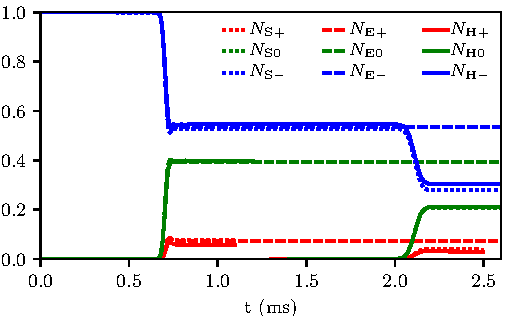
\includegraphics{figures/hidden_variables/hvsc/populations.pdf}
    }\\
    \subfloat[]{
    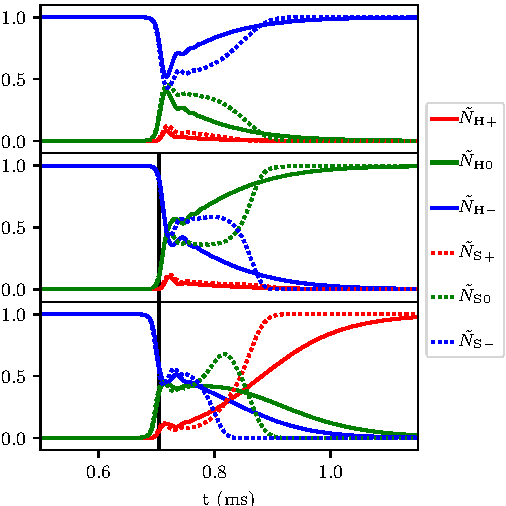
\includegraphics{figures/hidden_variables/hvsc_delta/populations_along_trajects.pdf}
    }
    \subfloat[]{
    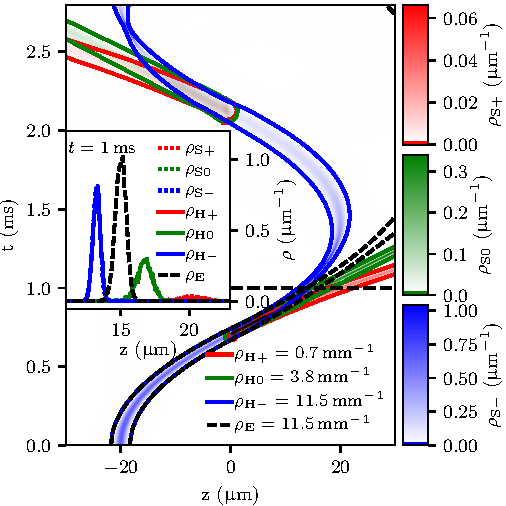
\includegraphics{figures/hidden_variables/hvsc/trajectories.pdf}
    }
    \caption{Scenario I results for the approximate Markovian decoherence hidden-variable semiclassical method (Section~\ref{sec:algo_markovian}), compared to the Schr\"odinger wave equation and Ehrenfest semiclassical method. (a) The populations $N$ in each spin projection state (denoted $N_\pm$, $N_0$ for $m_F=\pm 1$ and $m_F=0$ respectively) over time, obtained for the Schr\"odinger wave equation ($N_\up{S}$) by integration in the local basis over all space, for the Ehrenfest semiclassical model ($N_\up{E}$) as an expectation value over all semiclassical atoms' internal state vectors, and for the hidden-variable semiclassical method ($N_\up{H}$) as the proportion of atoms with the hidden variable specifying each state at each moment of time. The lines ending just after $1\unit{ms}$ is due to atoms/amplitude leaving the integration region. There is good agreement between all methods during the first approach of the field minimum, though the Ehrenfest trajectories do not make a second approach within the simulated interval. The remaining deviations between the Schr\"odinger and hidden-variable curves are within the random variation of the stochastic method. (b) The local state populations along specific trajectories corresponding to classical motion in $m_F=-1$ (top) for all time, switching to $m_F=0$ at the first field minimum (middle), and to $m_F=1$ (bottom). These were obtained by interpolation and normalisation of the Schr\"odinger wave equation results, and by selecting the semiclassical atoms making the chosen hidden-variable transitions closest to the field minimum (black lines). One trajectory resulting from the Ehrenfest model was chosen for comparison, its trajectory is close to those of the other two models until the field minimum, after which it diverges. This plot shows the shape of the decoherence curves and how our exponential approximation---while a poor fit---does have the correct timescale, and is better than the Ehrenfest method's absence of any decoherence. (c) Probability density of trajectories. Schr\"odinger wave equation results (shaded), and Ehrenfest and hidden-variable semiclassical results shown with a single contour line for a chosen density. Inset: The probability distributions at $1\unit{ms}$. There is good agreement between the hidden-variable semiclassical and Schr\"odinger wave equation results.}\label{fig:scenario_one_markovian}
\end{figure}
\restoregeometry}

\afterpage{
\newgeometry{left=1in,bottom=1.5in,right=1in,top=1.5in}
\begin{figure}
    % \centering
    \subfloat[]{
    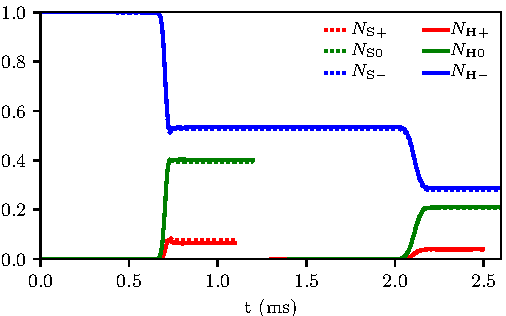
\includegraphics{figures/hidden_variables/hvsc_aux/populations.pdf}
    }\\
    \subfloat[]{
    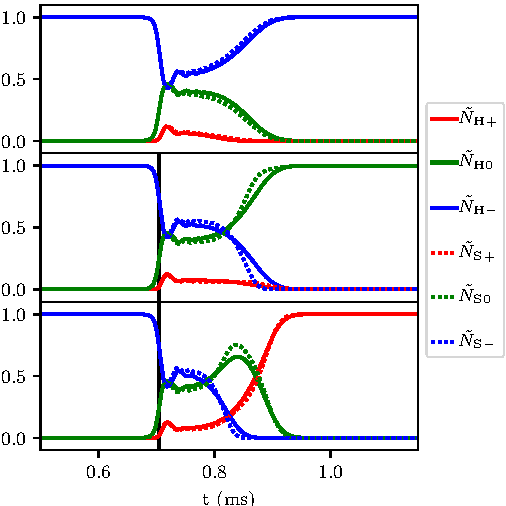
\includegraphics{figures/hidden_variables/hvsc_aux_delta/populations_along_trajects.pdf}
    }
    \subfloat[]{
    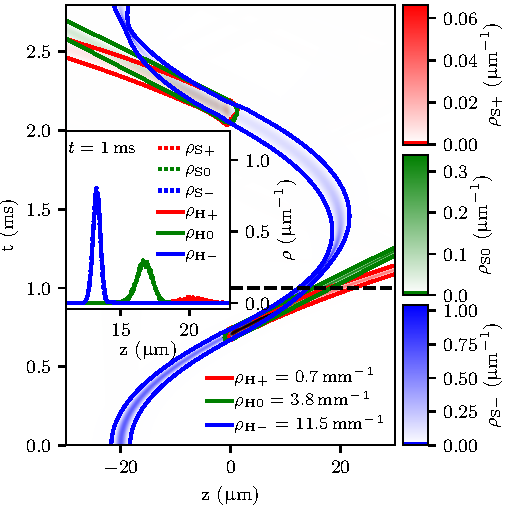
\includegraphics{figures/hidden_variables/hvsc_aux/trajectories.pdf}
    }
    \caption{Scenario I results for the mean-auxiliary-trajectories hidden-variable semiclassical method (Section~\ref{sec:algo_non_markovian}) compared to the Schr\"odinger wave equation (Ehrenfest results excluded from this and subsequent results plots for clarity). (a) As per~\figref{fig:scenario_one_markovian}. Once again, there is good agreement between all methods during the first approach of the field minimum, and good agreement between the hidden-variable semiclassical method during the second approach, though the Ehrenfest trajectories do not approach a second time. Again, the remaining deviation is within the range expected given the stochastic algorithm and could be reduced by increasing the sample size. (b) Populations after projecting onto specific classical trajectories, as and comparing with semiclassical atoms closest to those trajectories, as per~\figref{fig:scenario_one_markovian}. Here we see that the decoherence curves traced out by the auxiliary-trajectories method are in much closer agreement with the results of the Schr\"odinger wave equation than those of the Markovian model. Again, the discrepancies are within the statistical variation of the model; shown in each subplot is the atom that was closest to the given trajectory. (c). Probability density of trajectories of the two methods, as described in~\figref{fig:scenario_one_markovian}. Once again there is excellent agreement between the Schr\"odinger wave equation and hidden-variable semiclassical methods, with the Ehrenfest trajectories showing the expected unphysical behaviour.}\label{fig:scenario_one_aux}
\end{figure}
\restoregeometry}

\afterpage{
\newgeometry{left=1in,bottom=1.5in,right=1in,top=1.5in}
\begin{figure}
    % \centering
    \subfloat[]{
    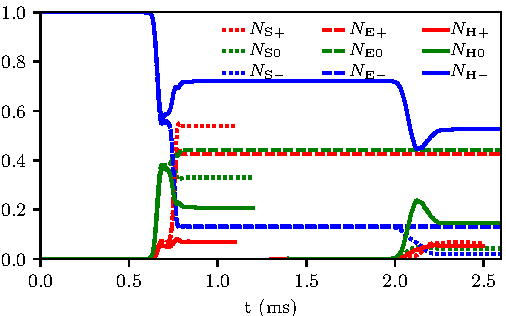
\includegraphics{figures/hidden_variables/hvsc_mirror/populations.pdf}
    }\\
    \subfloat[]{
    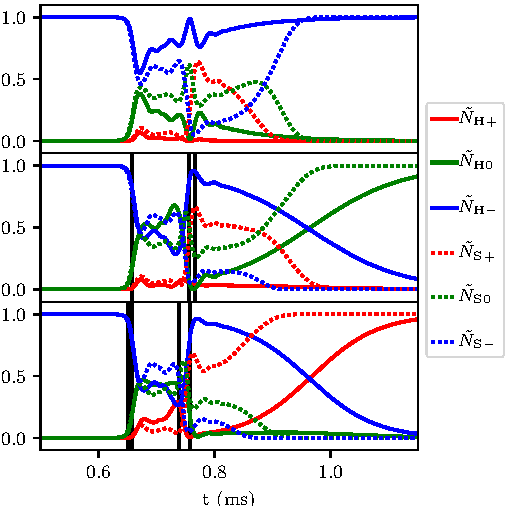
\includegraphics{figures/hidden_variables/hvsc_mirror_delta/populations_along_trajects.pdf}
    }
    \subfloat[]{
    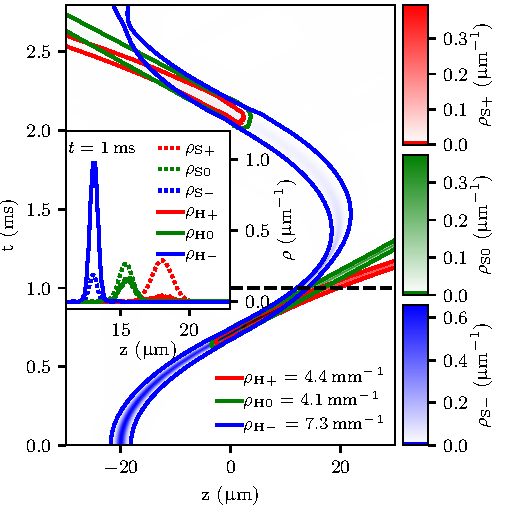
\includegraphics{figures/hidden_variables/hvsc_mirror/trajectories.pdf}
    }
    \caption{Scenario II results for the approximate Markovian decoherence hidden-variable semiclassical method (Section~\ref{sec:algo_markovian}) compared to the Schr\"odinger wave equation. All subfigures as described in~\figref{fig:scenario_one_markovian}. There are two minima in the magnetic field, closely spaced near $z=0$. Here we see the breakdown of the Markovian model in the presence of a second region of non-adiabatic coupling that the atoms encounter before they have fully decohered after the first. (a) The inaccurate modelling of decoherence has resulted in the wrong relative populations and phases between the states when the atom encounters the second region of coupling, leading to completely different populations after it emerges from the second field minimum. (b) Local populations along specific classical trajectories. Incorrect decoherence transients were inconsequential when there were no closely spaced field minima, but here the wrong decoherence results in the wrong initial conditions as the atom enter the region of non-adiabatic coupling near the second field minimum. If the minima were farther apart, the exponential decoherence would decay the system back to a single eigenstate, which would be correct. At shorter times, it matters whether the decoherence curves actually have the right shape. The semiclassical atoms near the centre of the wavepacket have very small population in $m_F=0$ and $m_F=-1$ states after the second region of coupling, as such there were no simulated atoms whose hidden variable remained in these two states after the first region of coupling. Plotted instead are results from atoms that made additional spin flips, but quickly transitioned back to the desired state. This can be seen as groups of multiple black lines indicating a number of closely spaced spin flips. As mentioned earlier, this is one disadvantage of Schr\"odinger theory: it often makes multiple transitions in a region of coupling in cases where Tully's fewest-switches algorithm would make only one, making it harder to pick out which atoms made certain transitions of interest. (c) Probability density of trajectories. The trajectories themselves are in excellent agreement with the Schr\"odinger wave equation---but there are the wrong proportion of atoms in each cluster of trajectories.}\label{fig:scenario_two_markovian}
\end{figure}
\restoregeometry}

\afterpage{
\newgeometry{left=1in,bottom=1.5in,right=1in,top=1.5in}
\begin{figure}
    % \centering
    \subfloat[]{
    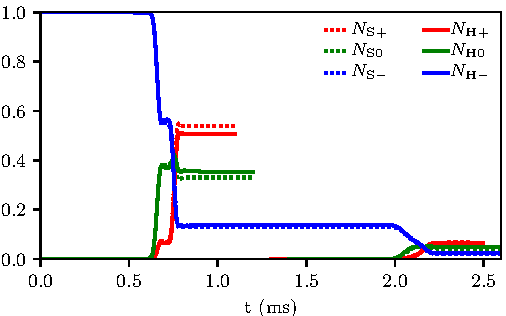
\includegraphics{figures/hidden_variables/hvsc_aux_mirror/populations.pdf}
    }\\
    \subfloat[]{
    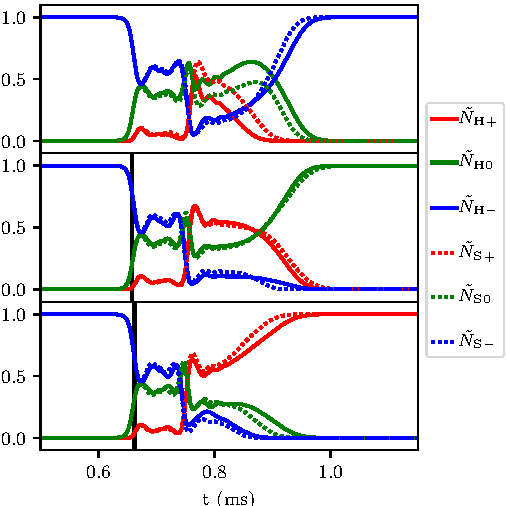
\includegraphics{figures/hidden_variables/hvsc_aux_mirror_delta/populations_along_trajects.pdf}
    }
    \subfloat[]{
    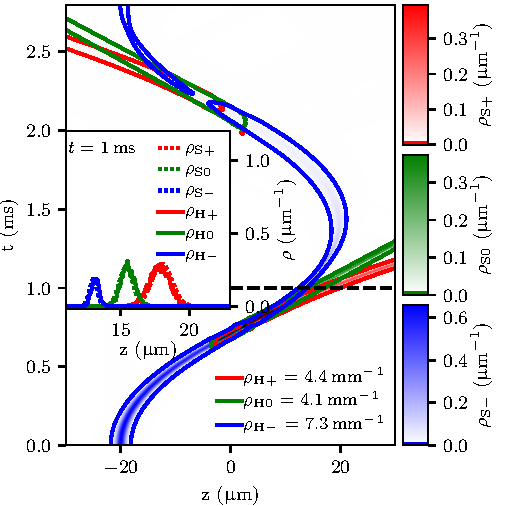
\includegraphics{figures/hidden_variables/hvsc_aux_mirror/trajectories.pdf}
    }
    \caption{Scenario II results for the mean-auxiliary-trajectories hidden-variable semiclassical method (Section~\ref{sec:algo_non_markovian}) compared to the Schr\"odinger wave equation. All subfigures as described in~\figref{fig:scenario_one_markovian}. (a) Here we see that the auxiliary-trajectories method of modelling decoherence leads to correct populations (again, within statistical error), even when there are two field minima closely spaced. (b) Here we see why: the decoherence curves match those of the Schr\"odinger wave equation in between the two field minima (identifiable by the two large vertical drops in the $m_F=-1$ population), providing the correct initial conditions as the atoms approach the second field minimum. (c) The trajectories and probability density functions agree well.}\label{fig:scenario_two_aux}
\end{figure}
\restoregeometry}

% \clearpage

\subsection{Gaussian projection results}

Here I demonstrate the difference between the above results, which use the Dirac delta based decoherence rates (Section~\ref{sec:dirac_deltas}), with what one obtains if projecting onto a Gaussian instead as originally proposed in Sections~\ref{sec:markovian_decoherence} and~\ref{sec:spawned_trajectories}. Here I only use the mean-auxiliary-trajectories method; though as argued in Section~\ref{sec:dirac_deltas}, the Markovian decoherence rate has its problems too when derived assuming Gaussian projections.

For these results I simulated scenario II, in which there are two closely spaced magnetic field minima, using two different decoherence rates. In the first, I take the decoherence rate $\gamma^\up{\textsc{mm}}_{ij}(t)$ given by~\eqref{eq:mm_decoherence_rate} at face value, velocity-space separation included. This leads to poor results as the decoherence is clearly too fast, as shown in~\figref{fig:very_bad_gamma}.

In the second, I make a similar change to that of Shenvi \emph{et al.}~\cite{doi:10.1063/1.3575588}, setting $\vec k_{ij} = 0$ for the relative wavenumber of the two Gaussian wavepackets in the decoherence factor~\eqref{eq:decoherence_factor}, and otherwise proceed as normal per Section~\ref{sec:decoherence_without_projection}. This gives a minimal-memory decoherence rate
\begin{align}
\gamma^\up{\textsc{mm}}_{ij}|_{\vec k_{ij} = 0}(t) = \frac{1}{4\sigma^2}\vec r_{ij}(t)\cdot\vec v_{ij}(t).
\end{align}
This leads to much better results, shown in~\figref{fig:bad_gamma} but still not as good as the Dirac delta based decoherence rate, shown in~\figref{fig:scenario_two_aux}. 

\afterpage{
\newgeometry{left=1in,bottom=1.5in,right=1in,top=1.5in}
\begin{figure}
    % \centering
    \subfloat[]{
    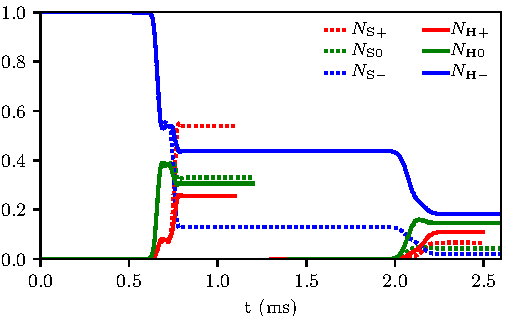
\includegraphics{figures/hidden_variables/hvsc_aux_mirror_very_bad_gamma/populations.pdf}
    }\\
    \subfloat[]{
    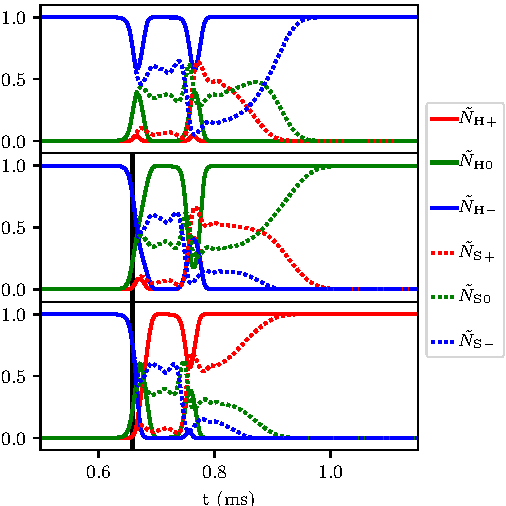
\includegraphics{figures/hidden_variables/hvsc_aux_mirror_very_bad_gamma_delta/populations_along_trajects.pdf}
    }
    \subfloat[]{
    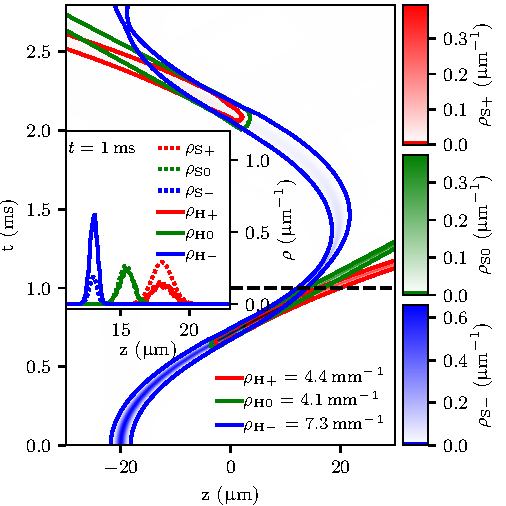
\includegraphics{figures/hidden_variables/hvsc_aux_mirror_very_bad_gamma/trajectories.pdf}
    }
    \caption{Scenario II results with the mean-auxiliary-trajectories hidden-variable semiclassical model (Section~\ref{sec:algo_non_markovian}), modified to use Gaussian-projection based decoherence rates, compared to the Schr\"odinger wave equation. All subplots as described in~\figref{fig:scenario_one_markovian}. (a) Populations after the first region of coupling are correct, but are clearly not correct after the second region of coupling. (b) We see that the cause of this is decoherence that is much too fast decoherence, with population of states other than that selected by the hidden variable decaying away at a rate as fast or faster than that at which it appears, leading to symmetrical profiles in population around the coupling regions. Of course, since this plot is comparing the state vector's local populations to those of the exact wavefunction along specific trajectories, and the decoherence model for this simulation is one based on projecting onto Gaussians rather than Dirac deltas centred exactly on the trajectory, we should not expect them to exactly agree (for that we would need to compare to projections of the exact wavefunctions onto Gaussians). However the disagreement is stark enough to make our point despite this. (c) As with the other results with poor modelling of decoherence, the trajectories are correct but the populations are not.}\label{fig:very_bad_gamma}
\end{figure}
\restoregeometry}

\afterpage{
\newgeometry{left=1in,bottom=1.5in,right=1in,top=1.5in}
\begin{figure}
    % \centering
    \subfloat[]{
    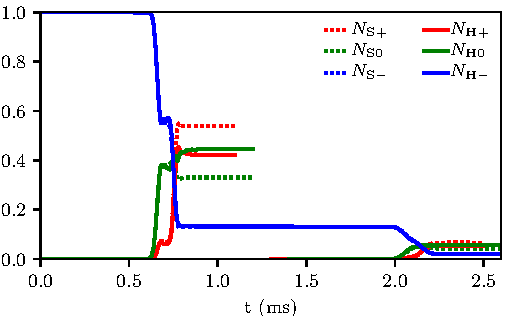
\includegraphics{figures/hidden_variables/hvsc_aux_mirror_bad_gamma/populations.pdf}
    }\\
    \subfloat[]{
    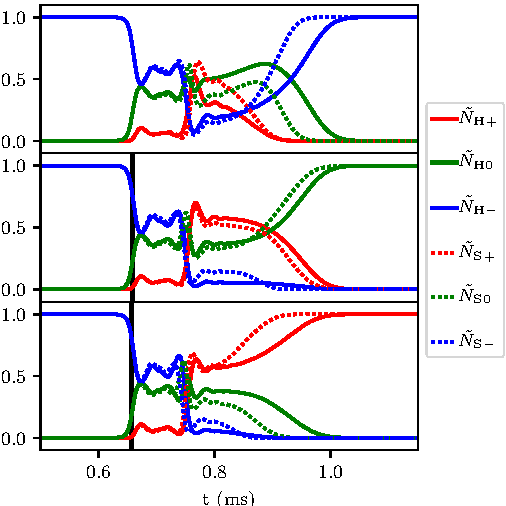
\includegraphics{figures/hidden_variables/hvsc_aux_mirror_bad_gamma_delta/populations_along_trajects.pdf}
    }
    \subfloat[]{
    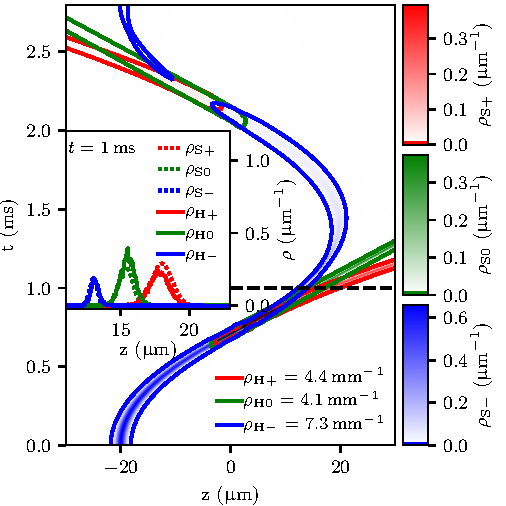
\includegraphics{figures/hidden_variables/hvsc_aux_mirror_bad_gamma/trajectories.pdf}
    }
    \caption{Scenario II results with Gaussian-projection based decoherence under the assumption of zero relative wavenumber between the Gaussians being projected onto each other when computing the decoherence rate. This decoherence rate $\gamma^\up{\textsc{mm}}_{ij}|_{\vec k_{ij} = 0}(t)$ is used with the mean-auxiliary-trajectories hidden-variable semiclassical model (Section~\ref{sec:algo_non_markovian}), and the results compared to the Schr\"odinger wave equation. All subplots as described in~\figref{fig:scenario_one_markovian}. (a) State populations are in much closer agreement with the Schr\"odinger wave equation results than when we did not set the relative wavenumber of the Gaussians to zero (\figref{fig:very_bad_gamma}). However, they are still not as accurate as our Dirac delta based decoherence model (\figref{fig:scenario_two_aux}). (b) As with~\figref{fig:very_bad_gamma}, we should not expect the local Schr\"odinger wave equation populations along the trajectories of the semiclassical atoms to agree with the state populations. However, for the three semiclassical atoms plotted (chosen as their trajectories were closest to the centre of the Gaussians and their transitions closest to the centre of the first region of coupling), they appear to agree quite well, including immediately after the second region of coupling. This may be a coincidence, or perhaps population transfers for atoms near the centre of the Gaussian are computed accurately with this decoherence model, but less accurately for atoms on other trajectories. (c). As usual, the trajectories are correct. We can see the minor error in populations in the inset, and it does not appear that the populations are more accurate in the centre as we just speculated. So any region of high accuracy in population transfer must be small enough to be hidden within the bins of the histogram, and is therefore not particularly of interest.}\label{fig:bad_gamma}
\end{figure}
\restoregeometry}

% \clearpage

\section{Discussion and conclusion}\label{sec:HVSC_discussion}

The methods presented in this chapter give acceptable results in different scenarios. The Markovian decoherence model (Section~\ref{sec:markovian_decoherence} and modifications in Section~\ref{sec:dirac_deltas}) is able to obtain accurate trajectories and state populations for semiclassical atoms in the case of non-adiabatic coupling regions that are encountered at intervals that are large compared to the decoherence time (Figure~\ref{fig:scenario_one_markovian}), but produces inaccurate populations if multiple coupling regions are encountered at smaller time intervals (Figure~\ref{fig:scenario_two_markovian}). The mean auxiliary trajectories method (Section~\ref{sec:spawned_trajectories} and modifications in Section~\ref{sec:dirac_deltas}) solves this problem by more accurately modelling dynamic decoherence curves, and is therefore able to obtain accurate trajectories and state populations even in the presence of multiple regions of coupling encountered at intervals comparable to the decoherence timescale (Figure~\ref{fig:scenario_two_aux}). Both methods are improvements over the Ehrenfest semiclassical method, which has no decoherence and no separation of trajectories, and over Tully's original model, which had separation of trajectories but no decoherence. 

The problem of velocity separation of wavepackets causing unexpected and undesired additional decoherence is resolved by instead modelling a projected state vector that is a projection of the multi-component wavefunction onto a Dirac delta---rather than a Gaussian wavepacket---equivalent to evaluating the wavefunction at a specific point in space following a classical trajectory over time (Section~\ref{sec:dirac_deltas}). The total multi-component wavefunction is still modelled as a collection of Gaussian wavepackets following classical trajectories. This is a more natural way to obtain state vectors that are statistically representative of the underlying multi-component wavefunctions we are approximating. As this is not based on wavepacket overlaps integrals, population in a state with a different phase gradient is not treated as having vanished merely because it has an inhomogeneous phase---instead we obtain some population, and some (perhaps rapidly varying) phase.

The above solution to the velocity separation problem, along with my method of averaging auxiliary trajectories in order to model only one trajectory per internal state of the atom, are modest improvements over similar methods such as that by Shenvi \emph{et al.}~\cite{doi:10.1063/1.3575588}. The decoherence rate that results when Shenvi \emph{et al.}~remove velocity separation from their decoherence calculation are still based on the overlap of two Gaussians, and is therefore still a kind of average over the entire wavepacket. The real part of the resulting decoherence rate is different from that presented here, based on Dirac deltas, by a factor of two, and lacks an imaginary part (velocity separation in my model still causes a phase shift). As I've argued, using the value at the centre of the wavepacket is more natural than averaging, as this gives you something closer to a value the wavefunction actually has at some point in space, and this is borne out by the simulation results in the previous section. This improvement is particularly relevant to cold-atom physics, as the velocity-separation problem only rears its head for large wavepackets, and thus low temperatures.

Schr\"odinger theory has not been applied to surface-hopping prior to this work, and I've shown in the results section of this chapter that it gives good results. However, as discussed in Section~\ref{sec:schrodinger_theory_numerics}, it is considerably expensive to compute transition probabilities from, though it can take as input arbitrary unitaries, allowing one to compute transition probabilities consistent with quantum evolution over arbitrary time intervals, rather than integrating infinitesimal transition probabilities over a finite time interval as with Tully's fewest-switches. 

The fact that Tully's fewest-switches algorithm gives smaller transition probabilities than Schr\"odinger theory (even though both are consistent with the quantum probabilities) makes it more desirable for use in a surface-hopping/hidden-variable semiclassical model. This is because every transition the hidden variable of a semiclassical atom makes is an opportunity for the atom to spend some time subject to a different potential. Even if the probability of the atom ending up in the right state is correct, the more potential surfaces it visits on its way there, the larger the variance in the integrated force it experienced will be, and hence the larger the variance in its final trajectory. A larger number of transitions also implies a larger variance in the number of atoms in each state (as given by their hidden variable), even though the expectation value might agree with the quantum populations. A `fewest-switches' algorithm is therefore likely to be the most accurate in this sense of reduced statistical variation. One final advantage of fewest hops in the context of my mean-auxiliary-trajectories method is that it means the algorithm will not discard as many auxiliary trajectories upon switching to them, resulting in possibly more accurate decoherence.

On that note, one could also imagine a variation of the method where an auxiliary trajectory is simply considered the main trajectory upon a transition, and not replaced by the previous main trajectory. In that case the number of hops would not influence whether the decoherence history was destroyed more than necessary.

Although the core idea of using a stochastically evolving variable to choose which classical force to subject a semiclassical atom to wasn't original, in rediscovering it I have identified that hidden-variable theories and hopping algorithms are in fact the same thing. With the ideas from the surface-hopping literature that my method previously lacked, and with my own improvements, the method has applications to a range of problems in cold atom physics, in simulating evaporative cooling, laser cooling, and other phenomena in cold atom physics whenever thermal atoms are subject to state-dependent forces. 